\documentclass[11pt]{article}

% Shared notes settings for Applied Machine Learning lectures (UPES).
% Keep this file free of \documentclass to allow reuse via \input.

\usepackage[utf8]{inputenc}
\usepackage[T1]{fontenc}
\usepackage{lmodern}          % scalable T1 fonts; without this pdflatex falls back
\input{glyphtounicode}        % to bitmapped EC Type 3 and the PDFs are neither
\pdfgentounicode=1            % searchable nor screen-reader friendly
\usepackage[a4paper,margin=1in]{geometry}
\usepackage{hyperref}
\usepackage{xurl}
\usepackage{booktabs}
\usepackage{amsmath}
\usepackage{amssymb}
\usepackage{listings}
\usepackage{xcolor}
\usepackage{enumitem}
\usepackage{parskip}

% Code listings (Python-oriented for this subject).
\lstset{
  language=Python,
  basicstyle=\ttfamily\small,
  keywordstyle=\color{blue},
  commentstyle=\color{gray},
  stringstyle=\color{teal},
  showstringspaces=false,
  columns=fullflexible,
  frame=single,
  framerule=0.2pt,
  breaklines=true
}

\setlist[itemize]{topsep=0.3em,itemsep=0.2em}
\setlist[enumerate]{topsep=0.3em,itemsep=0.2em}

% Simple per-section source line.
\newcommand{\notesources}[1]{\par\noindent{\small\color{gray}\textit{Sources:} \sloppy #1\par}}

% Unit-wise source strings for this subject (used by slides + notes).
% Path is relative to the lecture `latex/` folder (the compilation CWD).
\IfFileExists{../../../_shared/aml-sources.tex}{%
  % Source strings for Applied Machine Learning (CSAI2017P) — used by slides + notes.
% Prescribed texts and reference books are taken from the course syllabus.
% Support texts are the author-hosted open-access editions:
%   statlearning.com            (ISL with Python)
%   probml.github.io/pml-book   (Murphy, Probabilistic Machine Learning)
%   d2l.ai                      (Dive into Deep Learning)
%   mml-book.github.io          (Mathematics for Machine Learning)

\newcommand{\AMLRepoURL}{https://github.com/tali7c/Applied-Machine-Learning}

% --- prescribed -------------------------------------------------------------
\newcommand{\AMLPrescribed}{%
M\"uller and Guido, \textit{Introduction to Machine Learning with Python}, O'Reilly, 2016.;%
Bishop, \textit{Pattern Recognition and Machine Learning}, Springer, 2006.;%
Murphy, \textit{Machine Learning: A Probabilistic Perspective}, MIT Press, 2012.;%
Han, Kamber and Pei, \textit{Data Mining: Concepts and Techniques} (3e), Morgan Kaufmann, 2012.%
}

% --- unit-wise ---------------------------------------------------------------
\newcommand{\AMLUnitISources}{%
M\"uller and Guido, \textit{Introduction to Machine Learning with Python}, Ch. 1.;%
Bishop, \textit{Pattern Recognition and Machine Learning}, Ch. 1.;%
Murphy, \textit{Probabilistic Machine Learning: An Introduction}, MIT Press, 2022, Ch. 1.;%
Mitchell, \textit{Machine Learning}, McGraw Hill, 1997, Ch. 1.;%
Scikit-learn documentation, accessed 2026-08-04.%
}

\newcommand{\AMLUnitIISources}{%
Bishop, \textit{Pattern Recognition and Machine Learning}, \S1.5, \S4.3, \S7.1.;%
Zhang, Lipton, Li and Smola, \textit{Dive into Deep Learning}, \S3.4.;%
Shalev-Shwartz and Ben-David, \textit{Understanding Machine Learning}, Ch. 15.;%
Murphy, \textit{Probabilistic Machine Learning: An Introduction}, Ch. 5.%
}

\newcommand{\AMLUnitIIISources}{%
Zhang, Lipton, Li and Smola, \textit{Dive into Deep Learning}, Ch. 12 (Optimization Algorithms).;%
Deisenroth, Faisal and Ong, \textit{Mathematics for Machine Learning}, Ch. 7.;%
Kingma and Ba, ``Adam: A Method for Stochastic Optimization,'' ICLR 2015.;%
Ruder, ``An overview of gradient descent optimization algorithms,'' arXiv:1609.04747, 2016.%
}

\newcommand{\AMLUnitIVSources}{%
Han, Kamber and Pei, \textit{Data Mining: Concepts and Techniques} (3e), Ch. 3.;%
M\"uller and Guido, \textit{Introduction to Machine Learning with Python}, Ch. 3--4.;%
James, Witten, Hastie, Tibshirani and Taylor, \textit{An Introduction to Statistical Learning with Python}, Ch. 5--6, 12.;%
Scikit-learn documentation (preprocessing, model selection), accessed 2026-08-04.%
}

\newcommand{\AMLUnitVSources}{%
James et al., \textit{An Introduction to Statistical Learning with Python}, Ch. 3--6.;%
Bishop, \textit{Pattern Recognition and Machine Learning}, Ch. 3.;%
Deisenroth, Faisal and Ong, \textit{Mathematics for Machine Learning}, Ch. 9.;%
M\"uller and Guido, \textit{Introduction to Machine Learning with Python}, \S2.3.%
}

\newcommand{\AMLUnitVISources}{%
Han, Kamber and Pei, \textit{Data Mining: Concepts and Techniques} (3e), Ch. 8--9.;%
James et al., \textit{An Introduction to Statistical Learning with Python}, Ch. 8--9.;%
Bishop, \textit{Pattern Recognition and Machine Learning}, Ch. 4--5, 7, 14.;%
Zhang et al., \textit{Dive into Deep Learning}, Ch. 5.%
}

\newcommand{\AMLUnitVIISources}{%
Han, Kamber and Pei, \textit{Data Mining: Concepts and Techniques} (3e), Ch. 10.;%
James et al., \textit{An Introduction to Statistical Learning with Python}, Ch. 12.;%
M\"uller and Guido, \textit{Introduction to Machine Learning with Python}, \S3.5.;%
Ester, Kriegel, Sander and Xu, ``A density-based algorithm for discovering clusters (DBSCAN),'' KDD 1996.%
}

\newcommand{\AMLLabSources}{%
M\"uller and Guido, \textit{Introduction to Machine Learning with Python}, companion notebooks.;%
McKinney, \textit{Python for Data Analysis} (3e), O'Reilly, 2022.;%
Scikit-learn user guide, accessed 2026-08-04.;%
Matplotlib and Seaborn documentation, accessed 2026-08-04.%
}
%
}{%
  % Faculty copies live under `private/` so their compile CWD is different.
  \IfFileExists{../../../../public/_shared/aml-sources.tex}{%
    % Source strings for Applied Machine Learning (CSAI2017P) — used by slides + notes.
% Prescribed texts and reference books are taken from the course syllabus.
% Support texts are the author-hosted open-access editions:
%   statlearning.com            (ISL with Python)
%   probml.github.io/pml-book   (Murphy, Probabilistic Machine Learning)
%   d2l.ai                      (Dive into Deep Learning)
%   mml-book.github.io          (Mathematics for Machine Learning)

\newcommand{\AMLRepoURL}{https://github.com/tali7c/Applied-Machine-Learning}

% --- prescribed -------------------------------------------------------------
\newcommand{\AMLPrescribed}{%
M\"uller and Guido, \textit{Introduction to Machine Learning with Python}, O'Reilly, 2016.;%
Bishop, \textit{Pattern Recognition and Machine Learning}, Springer, 2006.;%
Murphy, \textit{Machine Learning: A Probabilistic Perspective}, MIT Press, 2012.;%
Han, Kamber and Pei, \textit{Data Mining: Concepts and Techniques} (3e), Morgan Kaufmann, 2012.%
}

% --- unit-wise ---------------------------------------------------------------
\newcommand{\AMLUnitISources}{%
M\"uller and Guido, \textit{Introduction to Machine Learning with Python}, Ch. 1.;%
Bishop, \textit{Pattern Recognition and Machine Learning}, Ch. 1.;%
Murphy, \textit{Probabilistic Machine Learning: An Introduction}, MIT Press, 2022, Ch. 1.;%
Mitchell, \textit{Machine Learning}, McGraw Hill, 1997, Ch. 1.;%
Scikit-learn documentation, accessed 2026-08-04.%
}

\newcommand{\AMLUnitIISources}{%
Bishop, \textit{Pattern Recognition and Machine Learning}, \S1.5, \S4.3, \S7.1.;%
Zhang, Lipton, Li and Smola, \textit{Dive into Deep Learning}, \S3.4.;%
Shalev-Shwartz and Ben-David, \textit{Understanding Machine Learning}, Ch. 15.;%
Murphy, \textit{Probabilistic Machine Learning: An Introduction}, Ch. 5.%
}

\newcommand{\AMLUnitIIISources}{%
Zhang, Lipton, Li and Smola, \textit{Dive into Deep Learning}, Ch. 12 (Optimization Algorithms).;%
Deisenroth, Faisal and Ong, \textit{Mathematics for Machine Learning}, Ch. 7.;%
Kingma and Ba, ``Adam: A Method for Stochastic Optimization,'' ICLR 2015.;%
Ruder, ``An overview of gradient descent optimization algorithms,'' arXiv:1609.04747, 2016.%
}

\newcommand{\AMLUnitIVSources}{%
Han, Kamber and Pei, \textit{Data Mining: Concepts and Techniques} (3e), Ch. 3.;%
M\"uller and Guido, \textit{Introduction to Machine Learning with Python}, Ch. 3--4.;%
James, Witten, Hastie, Tibshirani and Taylor, \textit{An Introduction to Statistical Learning with Python}, Ch. 5--6, 12.;%
Scikit-learn documentation (preprocessing, model selection), accessed 2026-08-04.%
}

\newcommand{\AMLUnitVSources}{%
James et al., \textit{An Introduction to Statistical Learning with Python}, Ch. 3--6.;%
Bishop, \textit{Pattern Recognition and Machine Learning}, Ch. 3.;%
Deisenroth, Faisal and Ong, \textit{Mathematics for Machine Learning}, Ch. 9.;%
M\"uller and Guido, \textit{Introduction to Machine Learning with Python}, \S2.3.%
}

\newcommand{\AMLUnitVISources}{%
Han, Kamber and Pei, \textit{Data Mining: Concepts and Techniques} (3e), Ch. 8--9.;%
James et al., \textit{An Introduction to Statistical Learning with Python}, Ch. 8--9.;%
Bishop, \textit{Pattern Recognition and Machine Learning}, Ch. 4--5, 7, 14.;%
Zhang et al., \textit{Dive into Deep Learning}, Ch. 5.%
}

\newcommand{\AMLUnitVIISources}{%
Han, Kamber and Pei, \textit{Data Mining: Concepts and Techniques} (3e), Ch. 10.;%
James et al., \textit{An Introduction to Statistical Learning with Python}, Ch. 12.;%
M\"uller and Guido, \textit{Introduction to Machine Learning with Python}, \S3.5.;%
Ester, Kriegel, Sander and Xu, ``A density-based algorithm for discovering clusters (DBSCAN),'' KDD 1996.%
}

\newcommand{\AMLLabSources}{%
M\"uller and Guido, \textit{Introduction to Machine Learning with Python}, companion notebooks.;%
McKinney, \textit{Python for Data Analysis} (3e), O'Reilly, 2022.;%
Scikit-learn user guide, accessed 2026-08-04.;%
Matplotlib and Seaborn documentation, accessed 2026-08-04.%
}
%
  }{%
    % Question papers live at `private/<family>/<instrument>/`.
    \IfFileExists{../../../public/_shared/aml-sources.tex}{%
      % Source strings for Applied Machine Learning (CSAI2017P) — used by slides + notes.
% Prescribed texts and reference books are taken from the course syllabus.
% Support texts are the author-hosted open-access editions:
%   statlearning.com            (ISL with Python)
%   probml.github.io/pml-book   (Murphy, Probabilistic Machine Learning)
%   d2l.ai                      (Dive into Deep Learning)
%   mml-book.github.io          (Mathematics for Machine Learning)

\newcommand{\AMLRepoURL}{https://github.com/tali7c/Applied-Machine-Learning}

% --- prescribed -------------------------------------------------------------
\newcommand{\AMLPrescribed}{%
M\"uller and Guido, \textit{Introduction to Machine Learning with Python}, O'Reilly, 2016.;%
Bishop, \textit{Pattern Recognition and Machine Learning}, Springer, 2006.;%
Murphy, \textit{Machine Learning: A Probabilistic Perspective}, MIT Press, 2012.;%
Han, Kamber and Pei, \textit{Data Mining: Concepts and Techniques} (3e), Morgan Kaufmann, 2012.%
}

% --- unit-wise ---------------------------------------------------------------
\newcommand{\AMLUnitISources}{%
M\"uller and Guido, \textit{Introduction to Machine Learning with Python}, Ch. 1.;%
Bishop, \textit{Pattern Recognition and Machine Learning}, Ch. 1.;%
Murphy, \textit{Probabilistic Machine Learning: An Introduction}, MIT Press, 2022, Ch. 1.;%
Mitchell, \textit{Machine Learning}, McGraw Hill, 1997, Ch. 1.;%
Scikit-learn documentation, accessed 2026-08-04.%
}

\newcommand{\AMLUnitIISources}{%
Bishop, \textit{Pattern Recognition and Machine Learning}, \S1.5, \S4.3, \S7.1.;%
Zhang, Lipton, Li and Smola, \textit{Dive into Deep Learning}, \S3.4.;%
Shalev-Shwartz and Ben-David, \textit{Understanding Machine Learning}, Ch. 15.;%
Murphy, \textit{Probabilistic Machine Learning: An Introduction}, Ch. 5.%
}

\newcommand{\AMLUnitIIISources}{%
Zhang, Lipton, Li and Smola, \textit{Dive into Deep Learning}, Ch. 12 (Optimization Algorithms).;%
Deisenroth, Faisal and Ong, \textit{Mathematics for Machine Learning}, Ch. 7.;%
Kingma and Ba, ``Adam: A Method for Stochastic Optimization,'' ICLR 2015.;%
Ruder, ``An overview of gradient descent optimization algorithms,'' arXiv:1609.04747, 2016.%
}

\newcommand{\AMLUnitIVSources}{%
Han, Kamber and Pei, \textit{Data Mining: Concepts and Techniques} (3e), Ch. 3.;%
M\"uller and Guido, \textit{Introduction to Machine Learning with Python}, Ch. 3--4.;%
James, Witten, Hastie, Tibshirani and Taylor, \textit{An Introduction to Statistical Learning with Python}, Ch. 5--6, 12.;%
Scikit-learn documentation (preprocessing, model selection), accessed 2026-08-04.%
}

\newcommand{\AMLUnitVSources}{%
James et al., \textit{An Introduction to Statistical Learning with Python}, Ch. 3--6.;%
Bishop, \textit{Pattern Recognition and Machine Learning}, Ch. 3.;%
Deisenroth, Faisal and Ong, \textit{Mathematics for Machine Learning}, Ch. 9.;%
M\"uller and Guido, \textit{Introduction to Machine Learning with Python}, \S2.3.%
}

\newcommand{\AMLUnitVISources}{%
Han, Kamber and Pei, \textit{Data Mining: Concepts and Techniques} (3e), Ch. 8--9.;%
James et al., \textit{An Introduction to Statistical Learning with Python}, Ch. 8--9.;%
Bishop, \textit{Pattern Recognition and Machine Learning}, Ch. 4--5, 7, 14.;%
Zhang et al., \textit{Dive into Deep Learning}, Ch. 5.%
}

\newcommand{\AMLUnitVIISources}{%
Han, Kamber and Pei, \textit{Data Mining: Concepts and Techniques} (3e), Ch. 10.;%
James et al., \textit{An Introduction to Statistical Learning with Python}, Ch. 12.;%
M\"uller and Guido, \textit{Introduction to Machine Learning with Python}, \S3.5.;%
Ester, Kriegel, Sander and Xu, ``A density-based algorithm for discovering clusters (DBSCAN),'' KDD 1996.%
}

\newcommand{\AMLLabSources}{%
M\"uller and Guido, \textit{Introduction to Machine Learning with Python}, companion notebooks.;%
McKinney, \textit{Python for Data Analysis} (3e), O'Reilly, 2022.;%
Scikit-learn user guide, accessed 2026-08-04.;%
Matplotlib and Seaborn documentation, accessed 2026-08-04.%
}
%
    }{%
      % Marking schemes live at `private/solutions/<family>/<id>/latex/`.
      \IfFileExists{../../../../../public/_shared/aml-sources.tex}{%
        % Source strings for Applied Machine Learning (CSAI2017P) — used by slides + notes.
% Prescribed texts and reference books are taken from the course syllabus.
% Support texts are the author-hosted open-access editions:
%   statlearning.com            (ISL with Python)
%   probml.github.io/pml-book   (Murphy, Probabilistic Machine Learning)
%   d2l.ai                      (Dive into Deep Learning)
%   mml-book.github.io          (Mathematics for Machine Learning)

\newcommand{\AMLRepoURL}{https://github.com/tali7c/Applied-Machine-Learning}

% --- prescribed -------------------------------------------------------------
\newcommand{\AMLPrescribed}{%
M\"uller and Guido, \textit{Introduction to Machine Learning with Python}, O'Reilly, 2016.;%
Bishop, \textit{Pattern Recognition and Machine Learning}, Springer, 2006.;%
Murphy, \textit{Machine Learning: A Probabilistic Perspective}, MIT Press, 2012.;%
Han, Kamber and Pei, \textit{Data Mining: Concepts and Techniques} (3e), Morgan Kaufmann, 2012.%
}

% --- unit-wise ---------------------------------------------------------------
\newcommand{\AMLUnitISources}{%
M\"uller and Guido, \textit{Introduction to Machine Learning with Python}, Ch. 1.;%
Bishop, \textit{Pattern Recognition and Machine Learning}, Ch. 1.;%
Murphy, \textit{Probabilistic Machine Learning: An Introduction}, MIT Press, 2022, Ch. 1.;%
Mitchell, \textit{Machine Learning}, McGraw Hill, 1997, Ch. 1.;%
Scikit-learn documentation, accessed 2026-08-04.%
}

\newcommand{\AMLUnitIISources}{%
Bishop, \textit{Pattern Recognition and Machine Learning}, \S1.5, \S4.3, \S7.1.;%
Zhang, Lipton, Li and Smola, \textit{Dive into Deep Learning}, \S3.4.;%
Shalev-Shwartz and Ben-David, \textit{Understanding Machine Learning}, Ch. 15.;%
Murphy, \textit{Probabilistic Machine Learning: An Introduction}, Ch. 5.%
}

\newcommand{\AMLUnitIIISources}{%
Zhang, Lipton, Li and Smola, \textit{Dive into Deep Learning}, Ch. 12 (Optimization Algorithms).;%
Deisenroth, Faisal and Ong, \textit{Mathematics for Machine Learning}, Ch. 7.;%
Kingma and Ba, ``Adam: A Method for Stochastic Optimization,'' ICLR 2015.;%
Ruder, ``An overview of gradient descent optimization algorithms,'' arXiv:1609.04747, 2016.%
}

\newcommand{\AMLUnitIVSources}{%
Han, Kamber and Pei, \textit{Data Mining: Concepts and Techniques} (3e), Ch. 3.;%
M\"uller and Guido, \textit{Introduction to Machine Learning with Python}, Ch. 3--4.;%
James, Witten, Hastie, Tibshirani and Taylor, \textit{An Introduction to Statistical Learning with Python}, Ch. 5--6, 12.;%
Scikit-learn documentation (preprocessing, model selection), accessed 2026-08-04.%
}

\newcommand{\AMLUnitVSources}{%
James et al., \textit{An Introduction to Statistical Learning with Python}, Ch. 3--6.;%
Bishop, \textit{Pattern Recognition and Machine Learning}, Ch. 3.;%
Deisenroth, Faisal and Ong, \textit{Mathematics for Machine Learning}, Ch. 9.;%
M\"uller and Guido, \textit{Introduction to Machine Learning with Python}, \S2.3.%
}

\newcommand{\AMLUnitVISources}{%
Han, Kamber and Pei, \textit{Data Mining: Concepts and Techniques} (3e), Ch. 8--9.;%
James et al., \textit{An Introduction to Statistical Learning with Python}, Ch. 8--9.;%
Bishop, \textit{Pattern Recognition and Machine Learning}, Ch. 4--5, 7, 14.;%
Zhang et al., \textit{Dive into Deep Learning}, Ch. 5.%
}

\newcommand{\AMLUnitVIISources}{%
Han, Kamber and Pei, \textit{Data Mining: Concepts and Techniques} (3e), Ch. 10.;%
James et al., \textit{An Introduction to Statistical Learning with Python}, Ch. 12.;%
M\"uller and Guido, \textit{Introduction to Machine Learning with Python}, \S3.5.;%
Ester, Kriegel, Sander and Xu, ``A density-based algorithm for discovering clusters (DBSCAN),'' KDD 1996.%
}

\newcommand{\AMLLabSources}{%
M\"uller and Guido, \textit{Introduction to Machine Learning with Python}, companion notebooks.;%
McKinney, \textit{Python for Data Analysis} (3e), O'Reilly, 2022.;%
Scikit-learn user guide, accessed 2026-08-04.;%
Matplotlib and Seaborn documentation, accessed 2026-08-04.%
}
%
      }{%
        % Source strings for Applied Machine Learning (CSAI2017P) — used by slides + notes.
% Prescribed texts and reference books are taken from the course syllabus.
% Support texts are the author-hosted open-access editions:
%   statlearning.com            (ISL with Python)
%   probml.github.io/pml-book   (Murphy, Probabilistic Machine Learning)
%   d2l.ai                      (Dive into Deep Learning)
%   mml-book.github.io          (Mathematics for Machine Learning)

\newcommand{\AMLRepoURL}{https://github.com/tali7c/Applied-Machine-Learning}

% --- prescribed -------------------------------------------------------------
\newcommand{\AMLPrescribed}{%
M\"uller and Guido, \textit{Introduction to Machine Learning with Python}, O'Reilly, 2016.;%
Bishop, \textit{Pattern Recognition and Machine Learning}, Springer, 2006.;%
Murphy, \textit{Machine Learning: A Probabilistic Perspective}, MIT Press, 2012.;%
Han, Kamber and Pei, \textit{Data Mining: Concepts and Techniques} (3e), Morgan Kaufmann, 2012.%
}

% --- unit-wise ---------------------------------------------------------------
\newcommand{\AMLUnitISources}{%
M\"uller and Guido, \textit{Introduction to Machine Learning with Python}, Ch. 1.;%
Bishop, \textit{Pattern Recognition and Machine Learning}, Ch. 1.;%
Murphy, \textit{Probabilistic Machine Learning: An Introduction}, MIT Press, 2022, Ch. 1.;%
Mitchell, \textit{Machine Learning}, McGraw Hill, 1997, Ch. 1.;%
Scikit-learn documentation, accessed 2026-08-04.%
}

\newcommand{\AMLUnitIISources}{%
Bishop, \textit{Pattern Recognition and Machine Learning}, \S1.5, \S4.3, \S7.1.;%
Zhang, Lipton, Li and Smola, \textit{Dive into Deep Learning}, \S3.4.;%
Shalev-Shwartz and Ben-David, \textit{Understanding Machine Learning}, Ch. 15.;%
Murphy, \textit{Probabilistic Machine Learning: An Introduction}, Ch. 5.%
}

\newcommand{\AMLUnitIIISources}{%
Zhang, Lipton, Li and Smola, \textit{Dive into Deep Learning}, Ch. 12 (Optimization Algorithms).;%
Deisenroth, Faisal and Ong, \textit{Mathematics for Machine Learning}, Ch. 7.;%
Kingma and Ba, ``Adam: A Method for Stochastic Optimization,'' ICLR 2015.;%
Ruder, ``An overview of gradient descent optimization algorithms,'' arXiv:1609.04747, 2016.%
}

\newcommand{\AMLUnitIVSources}{%
Han, Kamber and Pei, \textit{Data Mining: Concepts and Techniques} (3e), Ch. 3.;%
M\"uller and Guido, \textit{Introduction to Machine Learning with Python}, Ch. 3--4.;%
James, Witten, Hastie, Tibshirani and Taylor, \textit{An Introduction to Statistical Learning with Python}, Ch. 5--6, 12.;%
Scikit-learn documentation (preprocessing, model selection), accessed 2026-08-04.%
}

\newcommand{\AMLUnitVSources}{%
James et al., \textit{An Introduction to Statistical Learning with Python}, Ch. 3--6.;%
Bishop, \textit{Pattern Recognition and Machine Learning}, Ch. 3.;%
Deisenroth, Faisal and Ong, \textit{Mathematics for Machine Learning}, Ch. 9.;%
M\"uller and Guido, \textit{Introduction to Machine Learning with Python}, \S2.3.%
}

\newcommand{\AMLUnitVISources}{%
Han, Kamber and Pei, \textit{Data Mining: Concepts and Techniques} (3e), Ch. 8--9.;%
James et al., \textit{An Introduction to Statistical Learning with Python}, Ch. 8--9.;%
Bishop, \textit{Pattern Recognition and Machine Learning}, Ch. 4--5, 7, 14.;%
Zhang et al., \textit{Dive into Deep Learning}, Ch. 5.%
}

\newcommand{\AMLUnitVIISources}{%
Han, Kamber and Pei, \textit{Data Mining: Concepts and Techniques} (3e), Ch. 10.;%
James et al., \textit{An Introduction to Statistical Learning with Python}, Ch. 12.;%
M\"uller and Guido, \textit{Introduction to Machine Learning with Python}, \S3.5.;%
Ester, Kriegel, Sander and Xu, ``A density-based algorithm for discovering clusters (DBSCAN),'' KDD 1996.%
}

\newcommand{\AMLLabSources}{%
M\"uller and Guido, \textit{Introduction to Machine Learning with Python}, companion notebooks.;%
McKinney, \textit{Python for Data Analysis} (3e), O'Reilly, 2022.;%
Scikit-learn user guide, accessed 2026-08-04.;%
Matplotlib and Seaborn documentation, accessed 2026-08-04.%
}
%
      }%
    }%
  }%
}


\graphicspath{{../figures/}}

% This lecture pairs almost every paragraph with a listing and its output, so
% the default \medskipamount around each block adds up to several pages.
\lstset{aboveskip=3pt, belowskip=3pt}
\lstdefinestyle{amlout}{language={}, keepspaces=true,
  basicstyle=\ttfamily\footnotesize\color{black!80},
  backgroundcolor=\color{black!4}, frame=leftline, framerule=2pt,
  rulecolor=\color{black!25}, breaklines=true, columns=fullflexible,
  xleftmargin=8pt, aboveskip=2pt, belowskip=4pt, literate={-}{{-}}1}
\captionsetup{skip=4pt, font=small}
\renewcommand{\topfraction}{0.92}
\renewcommand{\bottomfraction}{0.75}
\renewcommand{\textfraction}{0.06}
\renewcommand{\floatpagefraction}{0.85}
\setlength{\floatsep}{6pt plus 2pt minus 2pt}
\setlength{\textfloatsep}{8pt plus 2pt minus 2pt}
\setlength{\intextsep}{8pt plus 2pt minus 2pt}

\newcommand{\bhat}{\hat\beta}
\newcommand{\XtX}{X^{\!\top}\!X}
\newcommand{\Xty}{X^{\!\top}y}

\title{Applied Machine Learning\\Unit 05 --- Lecture 12 Notes\\
       Regularization: Ridge and Lasso}
\author{Tofik Ali}
\date{Autumn 2026}

\begin{document}
\maketitle

\begin{keyidea}[Read this first]
These notes are written so that you can learn the material \emph{without}
having been in the lecture. Every concept is developed from scratch, every
number you see was produced by running the code shown beside it, and every
figure was generated from real computation rather than drawn by hand.

This lecture closes Unit V, and it is the answer to three problems the unit
raised and did not solve. \textbf{Over-fitting}: a model that reproduces the
training rows and generalises to nothing. \textbf{Multicollinearity}:
correlated columns that make $\XtX$ nearly singular, so the coefficients
become huge, opposite in sign and unstable. \textbf{Perfect separation}: a
logistic likelihood with no maximum, whose coefficients run away to infinity.

One idea answers all three. Stop asking for the model with the smallest
training error. Ask instead for a model with a small training error
\emph{and} small coefficients, and let a single dial decide the exchange rate
between them. That dial is $\lambda$, and it is not estimated by the fit --- it
is chosen from outside, by cross-validation.

The single structural fact to carry out of this lecture:
$\XtX + \lambda I$ is invertible for every $\lambda > 0$, \emph{whatever $X$
is}. Ridge regression therefore has an answer in situations where ordinary
least squares does not exist at all --- when two columns are exact copies,
when $p > n$, when the design is rank-deficient for any reason. That is not a
refinement of least squares. It is a change of kind.
\end{keyidea}

\tableofcontents
\medskip

% =========================================================================
\section{How to use these notes}
\label{sec:how}

Read in order. Section~\ref{sec:lasso} is written against
Section~\ref{sec:ridge} throughout, and Section~\ref{sec:bv} depends on both.
Everything here assumes the earlier Unit V material: least squares and the
normal equations, $R^2$, over-fitting, logistic regression, and multiple
regression with its multicollinearity problem. It also assumes the
cross-validation machinery from Unit IV.

There are four kinds of box. \textbf{Key idea} --- the one sentence to
remember a month from now. \textbf{Worked example} --- a calculation done by
hand, with small numbers, before any library is used. \textbf{Caution} --- the
specific mistake that section exists to prevent. \textbf{Try it yourself} ---
something to run, with the expected output given so you can check.

Code appears in a framed block, and directly beneath it a shaded block showing
what that code \emph{actually printed}. If you run it and get something
different, trust your machine and tell me.

\subsection{What you need}

\begin{lstlisting}
pip install numpy scipy scikit-learn matplotlib
\end{lstlisting}

Every number in these notes was produced with:

\begin{lstlisting}
import numpy, scipy, sklearn, matplotlib
print("numpy", numpy.__version__, "| scipy", scipy.__version__,
      "| sklearn", sklearn.__version__,
      "| matplotlib", matplotlib.__version__)
\end{lstlisting}
\begin{codeout}
numpy 2.2.6 | scipy 1.15.3 | sklearn 1.7.2 | matplotlib 3.10.9
\end{codeout}

\begin{sloppypar}
The running example is scikit-learn's bundled diabetes dataset, used in
\emph{both} of its forms. \texttt{load\_diabetes()} returns columns that have
already been centred and scaled, whereas
\texttt{load\_diabetes(scaled=False)} returns the original clinical units ---
and Section~\ref{sec:scale} needs those.
\end{sloppypar}

\begin{lstlisting}
from sklearn.datasets import load_breast_cancer, load_diabetes
dia = load_diabetes();  Xd, yd = dia.data, dia.target
Xr  = load_diabetes(scaled=False).data
\end{lstlisting}
\begin{codeout}
load_diabetes()              442 rows x 10 features, continuous target
load_diabetes(scaled=False)  same rows, ORIGINAL units
load_breast_cancer()         569 rows x 30 features, 2 classes
feature names: age, sex, bmi, bp, s1, s2, s3, s4, s5, s6
column standard deviations, scaled form : [0.0476 0.0476 0.0476 0.0476 0.0476 0.0476 0.0476 0.0476 0.0476 0.0476]
column standard deviations, raw form    : [13.09  0.5   4.41 13.82 34.57 30.38 12.92  1.29  0.52 11.48]
ratio widest / narrowest raw column: 69.3
no fetch_* call appears in this file
\end{codeout}

Everything else in these notes is a synthetic problem drawn from a single
seed, several of them deliberately with $p \ge n$.

\begin{keyidea}[One dataset, one seed --- the convention for this lecture]
Everything in these notes is computed from the \texttt{load\_diabetes} data
above and \textbf{one seed}. The seed is $\mathbf{0}$: every random number
generator is created as \texttt{np.random.default\_rng(0)}, every split and
every shuffle is \texttt{random\_state=0}, and every listing below that
draws, splits or resamples shows that argument rather than hiding it in a
helper.

Where a demonstration is genuinely \emph{about} run-to-run variation --- the
twenty draws of the $p>n$ problem in Section~\ref{sec:pgtn}, the thirty
bootstrap resamples in Section~\ref{sec:enet} --- the seeds are derived from
that same $0$ (\texttt{SEED}, \texttt{SEED+1}, \dots), so the spread is real
and the whole sweep still reproduces.

So every number printed in these notes reproduces \emph{exactly} if you run
the code as written. If you get something different, the difference is in your
code or your library versions, not in chance --- which is the only thing that
makes a printed number worth anything to you.
\end{keyidea}

\begin{caution}[Do not reach for \texttt{fetch\_*}]
Every \texttt{fetch\_*} loader downloads over HTTPS, and on the campus network
those downloads fail with a certificate error you cannot fix from your machine.
Nothing in this course depends on one: use the bundled loaders
(\texttt{load\_diabetes}, \texttt{load\_breast\_cancer}, \texttt{load\_iris},
\texttt{load\_wine}, \texttt{load\_digits}) or a fixed-seed synthetic set.
\end{caution}

\subsection{Learning outcomes}

By the end of this lecture you should be able to:

\begin{enumerate}[leftmargin=*]
  \item State the general form of a regularised objective,
    $\text{loss}(\beta) + \lambda\,\text{pen}(\beta)$, and explain why
    $\lambda$ is a hyper-parameter rather than a parameter (CO4).
  \item Derive the ridge closed form
    $\bhat = (\XtX + \lambda I)^{-1}\Xty$ from first principles, and prove
    that the matrix inverted is positive definite for every $\lambda > 0$
    (CO4).
  \item Compute a ridge estimate by hand on a small design at two or more
    values of $\lambda$, and verify it against \texttt{sklearn.linear\_model.Ridge}
    (CO4).
  \item Explain why the lasso has no closed-form solution, derive the
    soft-thresholding rule in the orthonormal case, and give both the
    algebraic and the geometric reason why the lasso produces exact zeros
    where ridge does not (CO4).
  \item Read a coefficient path, and use it to select a subset of predictors
    and to justify a value of $\lambda$ (CO4).
  \item Explain why regularised models require standardised predictors,
    quantify the cost of omitting the scaler, and state why the intercept is
    excluded from the penalty (CO4).
  \item Choose $\lambda$ by cross-validation, apply the one-standard-error
    rule, and report the resulting model with an honest held-out score (CO4).
  \item Decompose the expected test error of a ridge estimator into bias,
    variance and noise; show that some positive $\lambda$ always beats
    ordinary least squares; and apply this reasoning to a real problem (CO4).
  \item Describe the elastic net, its grouping effect, and the situation that
    motivates it (CO4).
\end{enumerate}

% =========================================================================
\section{Why regularization exists}
\label{sec:why}

\subsection{The general shape}

Every method in this lecture is a special case of one recipe:
\begin{equation}
  \bhat \;=\; \arg\min_\beta\ \underbrace{\text{loss}(\beta)}_{\text{fit the
  data}} \;+\; \lambda\,\underbrace{\text{pen}(\beta)}_{\text{stay small}},
  \qquad \lambda \ge 0 .
  \label{eq:general}
\end{equation}

At $\lambda = 0$ you get the unpenalised fit back exactly. As
$\lambda \to \infty$ the penalty dominates and every coefficient is driven to
zero, leaving the constant model. Everything of interest is in between, and
$\lambda$ is the dial.

\begin{keyidea}
$\lambda$ is not estimated by the fit. It is a \textbf{hyper-parameter},
chosen from outside by cross-validation --- which is why regularization could
not be taught before the validation material. A reported coefficient without
its $\lambda$ is meaningless.
\end{keyidea}

\subsection{Failure one: over-fitting}

Forty rows, thirty-eight columns, and only three of those columns carry any
signal. Ordinary least squares has just enough freedom to nearly interpolate.

\begin{lstlisting}
rng = np.random.default_rng(0)         # the one seed for this lecture
Xa = rng.normal(size=(40, 38))
beta_a = np.zeros(38);  beta_a[:3] = [3.0, -2.0, 1.5]
ya = Xa @ beta_a + rng.normal(0, 1.0, 40)
LinearRegression().fit(Xa, ya)
Ridge(alpha=10.0).fit(Xa, ya)
\end{lstlisting}
\begin{codeout}
(a) over-fitting     n=40  p=38
    OLS   train R2 +0.9997   test R2 +0.1470   ||beta||    5.075
    ridge train R2 +0.9336   test R2 +0.6598   ||beta||    2.432
\end{codeout}

Read the two rows against each other. Ridge fits the training data
\emph{worse} --- $0.9997$ down to $0.9336$ --- and fits $2000$ unseen rows more
than four times better. The coefficient vector halves in length. This is the
whole bargain of the lecture, in one table: give up training fit, buy test
fit.

\subsection{Failure two: multicollinearity}

Two columns that are the same underlying variable measured twice, with
correlation $0.99989$. The truth is $y = 2z$, so any split of the weight
between the two columns that sums to $2$ fits equally well.

\begin{lstlisting}
rng = np.random.default_rng(0)           # the one seed for this lecture
z  = rng.normal(size=100)
x1 = z + rng.normal(0, 0.01, 100);  x2 = z + rng.normal(0, 0.01, 100)
yb = 2.0 * z + rng.normal(0, 0.5, 100)
for b in range(5):                       # bootstrap resamples of the SAME rows
    idx = rng.integers(0, 100, 100)
    print(LinearRegression().fit(Xb[idx], yb[idx]).coef_,
          Ridge(alpha=1.0).fit(Xb[idx], yb[idx]).coef_)
\end{lstlisting}
\begin{codeout}
(b) multicollinearity  corr(x1,x2) = 0.999885
    OLS   coefficients [ 6.5628 -4.54  ]
    ridge coefficients [1.0549 0.9486]
    condition number of X'X: 1.692e+04
    the same fit on five bootstrap resamples of the same 100 rows:
       OLS [+11.0217,  -8.9539]   sum +2.0677      ridge [+1.1020, +0.9276]   sum +2.0297
       OLS [ +2.7446,  -0.6954]   sum +2.0492      ridge [+1.0332, +0.9985]   sum +2.0317
       OLS [ +6.7951,  -4.7408]   sum +2.0543      ridge [+1.0785, +0.9529]   sum +2.0315
       OLS [ +5.0355,  -3.0251]   sum +2.0105      ridge [+1.0354, +0.9583]   sum +1.9937
       OLS [ +7.5289,  -5.5234]   sum +2.0055      ridge [+1.0785, +0.9294]   sum +1.9867
\end{codeout}

Look first at the two \texttt{sum} columns: both are stable at about $2.0$,
because the sum is what the data actually determines. Now look at the pairs.
Ordinary least squares reports $(+11.02, -8.95)$ on one resample and
$(+2.74, -0.70)$ on the next --- the same population, the same $n$, a
completely different story about which variable matters. Ridge reports
$(1.10, 0.93)$ and $(1.03, 1.00)$.

\begin{keyidea}
Multicollinearity does not usually make the \emph{predictions} unstable. It
makes the \emph{coefficients} unstable, and therefore every interpretation you
build on them. Ridge stabilises them by refusing to let one column go large
and positive while its twin goes large and negative.
\end{keyidea}

\subsection{Failure three: perfect separation}

Six points, one feature, the two classes perfectly separated. The logistic
likelihood increases monotonically as the slope grows, so the maximum
likelihood estimate does not exist.

\begin{lstlisting}
xs = np.array([[-3.], [-2.], [-1.], [1.], [2.], [3.]]);  ys = [0,0,0,1,1,1]
for C in (1e10, 1.0, 0.01):
    print(C, LogisticRegression(C=C, max_iter=200000).fit(xs, ys).coef_)
\end{lstlisting}
\begin{codeout}
(c) perfect separation, 6 points, one feature
    C = 1e+10     penalty strength 1/C = 1e-10     fitted slope     8.3469
    C = 1         penalty strength 1/C = 1         fitted slope     1.1043
    C = 0.01      penalty strength 1/C = 100       fitted slope     0.0561
\end{codeout}

\begin{caution}[You have been using regularization since the logistic lecture]
\texttt{LogisticRegression} in scikit-learn is \textbf{L2-penalised by
default}, at \texttt{C=1}. The parameter \texttt{C} is $1/\lambda$: small
\texttt{C} means a strong penalty. Turn it effectively off
(\texttt{C=1e10}) and the slope climbs to $8.35$ and would keep climbing given
more iterations. On separated data the penalty is not a refinement --- it is
the only thing that makes an answer exist.
\end{caution}

% =========================================================================
\section{Ridge regression}
\label{sec:ridge}

\subsection{The objective, in two equivalent forms}

\textbf{Penalised form.} Minimise
\begin{equation}
  J(\beta) \;=\; (y - X\beta)^{\!\top}(y - X\beta)
    \;+\; \lambda\,\beta^{\!\top}\beta .
  \label{eq:ridgeobj}
\end{equation}

\textbf{Constrained form.} Minimise $(y - X\beta)^{\!\top}(y - X\beta)$
subject to $\|\beta\|_2^2 \le s$.

These are the same problem. For every $\lambda > 0$ there is an $s$ giving the
same solution, and vice versa; $\lambda$ is the Lagrange multiplier of the
constraint. The penalised form is what you compute with; the constrained form
is what you draw, and Section~\ref{sec:geometry} draws it.

Two conventions matter and are examinable.

\begin{enumerate}[leftmargin=*]
  \item \textbf{The intercept is not penalised.} The sum in
    Equation~\eqref{eq:ridgeobj} runs over $j = 1, \dots, p$, excluding
    $\beta_0$. Section~\ref{sec:intercept} shows what goes wrong otherwise.
  \item \textbf{The predictors are standardised first.} The penalty adds up
    $p$ squared coefficients as though they were in the same units. They are
    not, unless you make them so. Section~\ref{sec:scale} measures the damage.
\end{enumerate}

\subsection{Deriving the closed form}
\label{sec:derive}

Expand and differentiate. Using
$\frac{\partial}{\partial\beta}(y - X\beta)^{\!\top}(y - X\beta)
= -2X^{\!\top}(y - X\beta)$ and
$\frac{\partial}{\partial\beta}\lambda\beta^{\!\top}\beta = 2\lambda\beta$,

\begin{align}
  \nabla J(\beta) &= -2X^{\!\top}(y - X\beta) + 2\lambda\beta
    \;\stackrel{!}{=}\; 0 \notag\\[2pt]
  \Xty &= \XtX\beta + \lambda\beta \;=\; (\XtX + \lambda I)\beta \notag\\[2pt]
  \bhat^{\,\mathrm{ridge}} &= (\XtX + \lambda I)^{-1}\Xty .
  \label{eq:ridge}
\end{align}

Set $\lambda = 0$ and you recover $\bhat^{\,\mathrm{OLS}} = (\XtX)^{-1}\Xty$,
the normal equations from the least-squares lecture. Ridge is one extra term
on the diagonal --- and that one term is what the rest of this section is
about.

The Hessian is $\nabla^2 J = 2(\XtX + \lambda I)$, which the next subsection
shows is positive definite; the stationary point is therefore the unique
global minimum, and $J$ is strictly convex.

\subsection{The structural point: the inverse always exists}
\label{sec:invert}

\begin{keyidea}
For every $\lambda > 0$, the matrix $\XtX + \lambda I$ is positive definite,
and therefore invertible --- \textbf{whatever $X$ is}. Ridge regression has a
unique answer on designs where ordinary least squares has none.
\end{keyidea}

\textbf{Proof.} Let $v \ne 0$. Then
\begin{equation}
  v^{\!\top}(\XtX + \lambda I)v
  \;=\; v^{\!\top}\XtX v + \lambda v^{\!\top}v
  \;=\; \|Xv\|^2 + \lambda\|v\|^2 \;\ge\; \lambda\|v\|^2 \;>\; 0 .
  \label{eq:pd}
\end{equation}
The first term \emph{can} be zero --- $Xv = 0$ for some $v \ne 0$ is exactly
what it means for $\XtX$ to be singular --- but the second cannot be, because
$\lambda > 0$ and $v \ne 0$. A symmetric matrix with $v^{\!\top}Av > 0$ for
all $v \ne 0$ is positive definite, hence has strictly positive eigenvalues,
hence non-zero determinant, hence an inverse. $\square$

The eigenvalue version says the same thing more concretely. $\XtX$ is
symmetric positive semi-definite, so it has an orthonormal eigenbasis with
eigenvalues $d_1^2 \ge d_2^2 \ge \dots \ge d_p^2 \ge 0$, where the $d_j$ are
the singular values of $X$. Adding $\lambda I$ leaves the eigenvectors alone
and adds $\lambda$ to every eigenvalue:
\[
  \operatorname{eig}(\XtX + \lambda I) = \{\,d_j^2 + \lambda\,\}_{j=1}^{p},
  \qquad \text{all} > 0 .
\]
So the condition number falls from $d_1^2/d_p^2$ (which is $\infty$ when
$d_p = 0$) to $(d_1^2+\lambda)/(d_p^2+\lambda)$, which is finite always and
tends to $1$ as $\lambda$ grows. \textbf{Adding $\lambda$ to the diagonal
lifts every eigenvalue off the floor.}

\subsection{Worked: three numbers, one feature}
\label{sec:hand1}

\begin{worked}[Ridge by hand, at four values of $\lambda$]
Take $x = (1, 2, 2)^{\!\top}$ and $y = (2, 3, 5)^{\!\top}$, one feature, no
intercept. Then
\[
  \XtX = 1^2 + 2^2 + 2^2 = 9,
  \qquad
  \Xty = 1\cdot2 + 2\cdot3 + 2\cdot5 = 18 ,
\]
and Equation~\eqref{eq:ridge} is a division:
\[
  \bhat(\lambda) \;=\; \frac{18}{9 + \lambda}
  \;=\; \underbrace{2}_{\bhat^{\mathrm{OLS}}}
    \times \underbrace{\frac{9}{9+\lambda}}_{\text{shrinkage factor}} .
\]
\begin{center}
\begin{tabular}{@{}lrrrr@{}}
\toprule
$\lambda$ & $0$ & $1$ & $9$ & $81$\\
\midrule
$\bhat = 18/(9+\lambda)$ & $2.0000$ & $1.8000$ & $1.0000$ & $0.2000$\\
shrinkage factor $9/(9+\lambda)$ & $1.0000$ & $0.9000$ & $\mathbf{0.5000}$
  & $0.1000$\\
\bottomrule
\end{tabular}
\end{center}
At $\lambda = \XtX = 9$ the coefficient is halved exactly. That is worth
remembering: \textbf{$\lambda$ lives on the same scale as $\XtX$}, so whether
a given $\lambda$ is ``a lot'' depends entirely on the magnitude of the
numbers in $X$.
\end{worked}

\begin{lstlisting}
x = np.array([1., 2., 2.]);  y = np.array([2., 3., 5.])
for lam in (0., 1., 9., 81.):
    print(lam, Ridge(alpha=lam, fit_intercept=False)
                 .fit(x.reshape(-1, 1), y).coef_)
\end{lstlisting}
\begin{codeout}
x = [1, 2, 2]   y = [2, 3, 5]
X'X = 9     X'y = 18
  lambda     0   beta = 18 / ( 9 +  0) = 2.0000   shrinkage factor 1.0000
  lambda     1   beta = 18 / ( 9 +  1) = 1.8000   shrinkage factor 0.9000
  lambda     9   beta = 18 / ( 9 +  9) = 1.0000   shrinkage factor 0.5000
  lambda    81   beta = 18 / ( 9 + 81) = 0.2000   shrinkage factor 0.1000
check with sklearn Ridge(fit_intercept=False):
  lambda     0   sklearn coef_ = 2.0000
  lambda     1   sklearn coef_ = 1.8000
  lambda     9   sklearn coef_ = 1.0000
  lambda    81   sklearn coef_ = 0.2000
\end{codeout}

Four values, four exact matches. \texttt{Ridge} is
Equation~\eqref{eq:ridge} and nothing else.

\begin{caution}[\texttt{fit\_intercept=False} is doing real work here]
With the default \texttt{fit\_intercept=True}, scikit-learn centres $X$ and
$y$ before solving and then recovers $\beta_0$. The arithmetic above assumes
no centring, so the two only agree when you switch the intercept off. Whenever
you check a library against a hand calculation, check what it centres first.
\end{caution}

\begin{tryit}[Find the halving point yourself]
Take $x = (2, 2, 4)$ and $y = (3, 5, 8)$, one feature, no intercept. Compute
$\XtX$ and $\Xty$ on paper, write down $\bhat(\lambda)$, and find the $\lambda$
at which the coefficient is exactly half its least-squares value. Then check
with \texttt{Ridge(alpha=..., fit\_intercept=False)}. You should get
$\XtX = 24$, $\Xty = 48$, $\bhat^{\mathrm{OLS}} = 2$, and halving at
$\lambda = 24$. Question~\ref{q:hand1} continues this.
\end{tryit}

\begin{figure}[htbp]
  \centering
  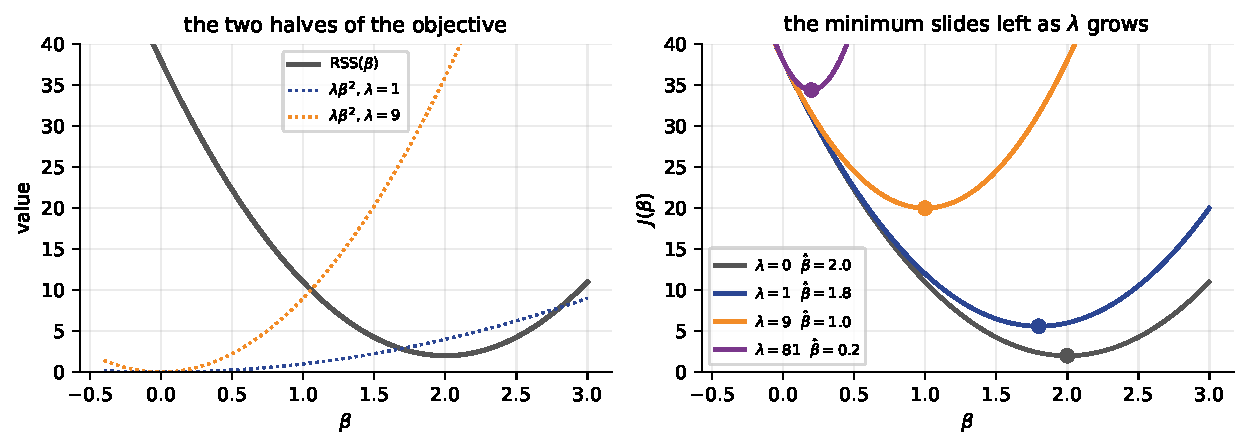
\includegraphics[width=0.92\textwidth]{handridge.pdf}
  \caption{The by-hand problem, drawn. Left: RSS is a parabola with its
  minimum at $\beta = 2$; $\lambda\beta^2$ is a parabola with its minimum at
  $\beta = 0$. Right: their sum for four values of $\lambda$, with the
  computed minimum marked. Adding a bowl centred at the origin drags the
  minimum towards the origin --- and, for finite $\lambda$, never all the way
  and never past it.}
  \label{fig:handridge}
\end{figure}

\subsection{Worked: a $2\times2$ inverse}
\label{sec:hand2}

\begin{worked}[The matrix version, still by hand]
\[
  X = \begin{pmatrix} 1 & 0\\ 0 & 1\\ 1 & 1\end{pmatrix},
  \qquad y = \begin{pmatrix}1\\2\\3\end{pmatrix},
  \qquad
  \XtX = \begin{pmatrix} 2 & 1\\ 1 & 2\end{pmatrix},
  \qquad \Xty = \begin{pmatrix}4\\5\end{pmatrix}.
\]
For a $2\times2$ matrix,
$\begin{pmatrix}a&b\\c&d\end{pmatrix}^{-1}
= \frac{1}{ad-bc}\begin{pmatrix}d&-b\\-c&a\end{pmatrix}$. At $\lambda = 1$:
\[
  \bhat = \begin{pmatrix}3&1\\1&3\end{pmatrix}^{-1}\begin{pmatrix}4\\5\end{pmatrix}
  = \frac{1}{8}\begin{pmatrix}3&-1\\-1&3\end{pmatrix}\begin{pmatrix}4\\5\end{pmatrix}
  = \frac{1}{8}\begin{pmatrix}12-5\\-4+15\end{pmatrix}
  = \frac{1}{8}\begin{pmatrix}7\\11\end{pmatrix}
  = \begin{pmatrix}0.8750\\1.3750\end{pmatrix}.
\]
\begin{center}
\begin{tabular}{@{}lccrr@{}}
\toprule
$\lambda$ & $\XtX + \lambda I$ & $\det$ & $\bhat$ & $\|\bhat\|_2$\\
\midrule
$0$ & $\left(\begin{smallmatrix}2&1\\1&2\end{smallmatrix}\right)$ & $3$
  & $(1.0000,\ 2.0000)$ & $2.2361$\\[3pt]
$1$ & $\left(\begin{smallmatrix}3&1\\1&3\end{smallmatrix}\right)$ & $8$
  & $(0.8750,\ 1.3750)$ & $1.6298$\\[3pt]
$3$ & $\left(\begin{smallmatrix}5&1\\1&5\end{smallmatrix}\right)$ & $24$
  & $(0.6250,\ 0.8750)$ & $1.0753$\\
\bottomrule
\end{tabular}
\end{center}
Notice that $\beta_1$ and $\beta_2$ do \emph{not} shrink by the same
proportion. Ridge is a uniform rescaling of the OLS vector only when $\XtX$
is a multiple of the identity.
\end{worked}

\begin{codeout}
  lambda 0   det   3.0   beta = [1.0000, 2.0000]   ||beta||_2 = 2.2361   ||beta||_1 = 3.0000
  lambda 1   det   8.0   beta = [0.8750, 1.3750]   ||beta||_2 = 1.6298   ||beta||_1 = 2.2500
  lambda 3   det  24.0   beta = [0.6250, 0.8750]   ||beta||_2 = 1.0753   ||beta||_1 = 1.5000
check with sklearn:
  lambda 0   sklearn coef_ = [1.0000, 2.0000]
  lambda 1   sklearn coef_ = [0.8750, 1.3750]
  lambda 3   sklearn coef_ = [0.6250, 0.8750]
\end{codeout}

\subsection{Ridge where OLS does not exist}
\label{sec:singular}

Now make the second column exactly twice the first. Nothing is
\emph{approximately} collinear here; the columns are linearly dependent.

\begin{lstlisting}
X5 = np.array([[1., 2.], [2., 4.], [3., 6.]])     # col 2 = 2 * col 1
y5 = np.array([1., 2., 3.])
np.linalg.inv(X5.T @ X5)
\end{lstlisting}
\begin{codeout}
X'X =
 [[14 28]
 [28 56]]
det(X'X) = 0.0     rank(X'X) = 1     eigenvalues [ 0. 70.]
np.linalg.inv(X'X) raises LinAlgError: Singular matrix
np.linalg.solve(X'X, X'y) raises: LinAlgError: Singular matrix
what LinearRegression does instead: lstsq gives the MINIMUM-NORM
  solution, not 'the' solution: [0.2 0.4]
\end{codeout}

Two things happened there and only one of them is obvious. The
\emph{formula} fails: $\det(\XtX) = 14\cdot56 - 28^2 = 784 - 784 = 0$, and
NumPy says so. But \texttt{LinearRegression} does \emph{not} fail. It calls
\texttt{lstsq}, which, when the solution is not unique, silently returns the
one with the smallest $\|\beta\|_2$ among the infinitely many that fit
perfectly. Nothing in the output tells you that choice was made.

\begin{caution}[\texttt{LinearRegression} never raises, so it never warns you]
On a rank-deficient design, \texttt{LinearRegression} returns a number and no
message. You must check the rank yourself:
\texttt{np.linalg.matrix\_rank(X)} against \texttt{X.shape[1]}. This matters
most in the $p > n$ case, where the design is \emph{always} rank-deficient.
\end{caution}

Ridge, on the same matrix:

\begin{codeout}
  lambda 1   X'X + 1 I =[[15 28] [28 57]]   det   71.0   eigenvalues [ 1. 71.]
             beta = [0.19718, 0.39437]     beta2 / beta1 = 2.0000
  lambda 4   X'X + 4 I =[[18 28] [28 60]]   det  296.0   eigenvalues [ 4. 74.]
             beta = [0.18919, 0.37838]     beta2 / beta1 = 2.0000
sklearn Ridge(alpha=1, fit_intercept=False).coef_ = [0.19718 0.39437]
\end{codeout}

The determinant went from $0$ to $71$ by adding $1$ to two diagonal entries,
and the eigenvalue that was $0$ is now exactly $\lambda$. Confirm the
$\lambda = 1$ answer by hand:
$\frac{1}{71}\left(\begin{smallmatrix}57&-28\\-28&15\end{smallmatrix}\right)
\left(\begin{smallmatrix}14\\28\end{smallmatrix}\right)
= \frac{1}{71}\left(\begin{smallmatrix}798-784\\-392+420\end{smallmatrix}\right)
= \frac{1}{71}\left(\begin{smallmatrix}14\\28\end{smallmatrix}\right)$.

And read $\beta_2/\beta_1 = 2.0000$: given two directions that are exact
copies, ridge splits the weight between them in proportion to their column
norms rather than choosing one. That is the grouping behaviour
Section~\ref{sec:enet} returns to.

\begin{figure}[htbp]
  \centering
  
\includegraphics[width=\textwidth]{collinear.pdf}
  \caption{The same three rows, drawn as a surface over the coefficient
  plane. Left: with a singular $\XtX$ the RSS contours are \emph{parallel
  straight lines} --- every point on the orange line $\beta_1 + 2\beta_2 = 1$
  fits all three rows exactly, so there is no unique minimiser, and
  \texttt{lstsq} breaks the tie by picking the point closest to the origin.
  Middle and right: adding $\lambda I$ closes the contours into ellipses. The
  smallest eigenvalue is exactly $\lambda$, so the ellipses get rounder as
  $\lambda$ grows.}
  \label{fig:collinear}
\end{figure}

\subsection{The $p > n$ case}
\label{sec:pgtn}

When there are more columns than rows, $\XtX$ is $p \times p$ but has rank at
most $n$, so it is \emph{always} singular. This is the regime of genomics, of
text, of any problem where measuring another variable is cheaper than
recruiting another subject.

\begin{lstlisting}
rng = np.random.default_rng(0)         # the one seed for this lecture
X6 = rng.normal(size=(50, 200))        # n = 50, p = 200
beta6 = np.zeros(200);  beta6[:5] = [4.0, -3.0, 2.5, 2.0, -1.5]
y6 = X6 @ beta6 + rng.normal(0, 1.0, 50)
\end{lstlisting}
\begin{codeout}
n = 50 rows, p = 200 columns
rank(X'X) = 50 of 200 -- X'X is singular by construction
number of zero eigenvalues of X'X: 150
smallest eigenvalue of X'X       : -1.812e-13
smallest eigenvalue of X'X + 10I : 1.000e+01
  OLS (lstsq min-norm)   train R2 +1.0000  test R2 +0.2831  ||beta||    3.178  nonzero 200
  Ridge alpha=10         train R2 +0.9974  test R2 +0.2792  ||beta||    2.998  nonzero 200
  Ridge, CV alpha 0.1    train R2 +1.0000  test R2 +0.2831  ||beta||    3.176  nonzero 200
  Lasso, CV alpha 0.215  train R2 +0.9807  test R2 +0.9294  ||beta||    5.268  nonzero  20
lasso kept 20 columns; the 5 truly non-zero ones are [0,1,2,3,4]
  are all five in the kept set? True
true coefficients       [ 4.  -3.   2.5  2.  -1.5]
lasso estimates there   [ 3.532 -2.934  1.912  1.284 -0.919]
ridge estimates there   [ 1.021 -0.937  0.561  0.464 -0.255]
\end{codeout}

Note the smallest eigenvalue: $-1.8\times10^{-13}$. It is not merely small,
it is \emph{negative}, which is arithmetically impossible for
$\XtX$ --- floating point has rounded a true zero the wrong way. Adding
$\lambda = 10$ makes it exactly $10$.

Two honest readings of this table.

\emph{First}, ``OLS'' here is not OLS. The minimum-norm solution
\texttt{lstsq} returns is precisely the limit of ridge as
$\lambda \to 0^{+}$:

\begin{codeout}
what lstsq actually returned: the MINIMUM-NORM solution, which is
exactly the limit of ridge as lambda -> 0:
   alpha 1e-03   max |ridge - lstsq| 6.486e-06   ||ridge|| 3.1907  ||lstsq|| 3.1907
   alpha 1e-06   max |ridge - lstsq| 6.486e-09   ||ridge|| 3.1907  ||lstsq|| 3.1907
   alpha 1e-09   max |ridge - lstsq| 6.487e-12   ||ridge|| 3.1907  ||lstsq|| 3.1907
so 'OLS' at p > n is not OLS. numpy silently regularised for you.
\end{codeout}

Agreement to $6\times10^{-12}$. Every time you fit ``ordinary least squares''
with more columns than rows, you are fitting a regularised estimator and
calling it something else.

\emph{Second}, on this problem ridge does essentially nothing and the lasso
is transformative: $0.2831 \to 0.9294$, recovering all five real columns with
estimates close to the truth. Look at what cross-validation chose for ridge:
$\alpha = 0.1$, the smallest value on the grid, reproducing the minimum-norm
fit to four decimals. Given a free choice of penalty strength, ridge declined
to use one. The reason is that the truth here is \emph{sparse}, and
Section~\ref{sec:lasso} is about the penalty built for that.

\subsubsection*{Where ridge earns its keep instead}

Change the problem so that the columns are correlated (driven by five latent
factors) and \emph{all} the coefficients are non-zero. Now no subset of
columns is the right answer, so the lasso has nothing to select.

\begin{lstlisting}
def dense_correlated(seed):            # seed = SEED, then SEED+1, SEED+2, ...
    g = np.random.default_rng(seed)
    load = g.normal(size=(5, 100)) / np.sqrt(5)      # five latent factors
    beta = g.normal(0, 0.4, 100)                     # every column matters
    ...
\end{lstlisting}
\begin{codeout}
n = 50, p = 100, columns driven by 5 latent factors (rho = 0.9),
and ALL 100 coefficients are non-zero.
mean |correlation| between distinct columns: 0.3370
  OLS (lstsq min-norm)     train R2 +1.0000  test R2 +0.4183   nonzero 100
  Ridge, CV alpha 5.2      train R2 +0.9469  test R2 +0.6303   nonzero 100
  Lasso, CV alpha 0.152    train R2 +0.8298  test R2 +0.6618   nonzero  14
one draw settles nothing at n = 50. repeating over 20 draws,
seeds SEED..SEED+19:
  mean test R2   OLS +0.4446   ridge +0.6532   lasso +0.6443
  worst OLS draw -0.4915; OLS is worse than predicting the mean in 1 of 20 draws
  ridge beats OLS in 19 of 20 draws, lasso in 16 of 20
\end{codeout}

Read the two halves of that output in order, because the second half is the
more important one.

On \emph{this} draw, ridge lifts the min-norm fit from $0.4183$ to $0.6303$
and the lasso, with only $14$ of the $100$ columns, edges ahead of both at
$0.6618$. That last fact is inconvenient for the tidy story you were about to
be told, so here is the honest version instead. At $n = 50$ with $p = 100$ the
minimum-norm fit is so unstable that a single draw can be made to say almost
anything: across twenty draws OLS ranged from $-0.4915$ to well above $0.7$.
Quoting the draw that suits you is not evidence, it is selection.

Across the twenty draws the pattern that does hold is this. Ridge beats the
unpenalised fit in $19$ of $20$ draws and averages $0.6532$ against OLS's
$0.4446$ --- a large, consistent gain. Ridge also beats the lasso, but only in
$16$ of $20$ draws, and on the average by the gap between $0.6532$ and
$0.6443$, which is nothing. That is
the true size of the effect: on a dense correlated truth ridge is the better
\emph{default}, not the certain winner.

\begin{keyidea}
Sparse truth $\to$ lasso wins, and wins hugely ($0.9294$ against $0.2831$).
Dense, correlated truth $\to$ ridge wins on average, and only narrowly
($0.6532$ against $0.6443$, in $16$ draws out of $20$). Neither penalty
dominates the other, you cannot tell which regime you are in by looking at the
data, and one draw of a $p > n$ problem is not an experiment. That is what
cross-validation, and repetition, are for.
\end{keyidea}

\begin{figure}[htbp]
  \centering
  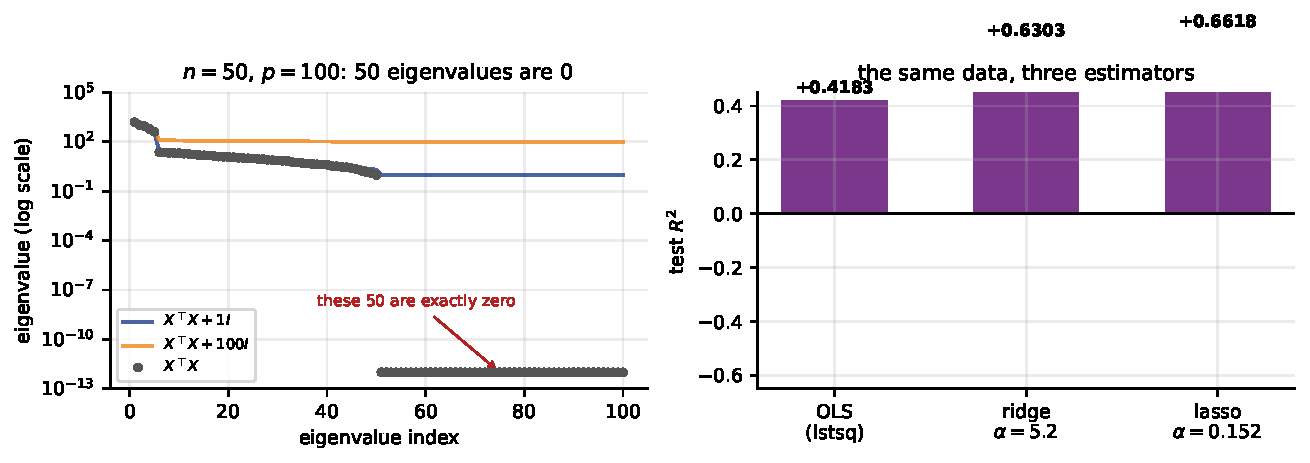
\includegraphics[width=0.95\textwidth]{pgtn.pdf}
  \caption{Left: the eigenvalues of $\XtX$ for $n = 50$, $p = 100$, on a log
  scale. Fifty are exactly zero and are plotted on the floor of the axis
  because $\log 0$ does not exist. Adding $\lambda I$ raises the entire
  spectrum by $\lambda$, which matters only where the spectrum was near the
  floor. Right: what that is worth on $2000$ held-out rows.}
  \label{fig:pgtn}
\end{figure}

\subsection{What ridge does direction by direction}
\label{sec:svd}

There is a cleaner way to see ridge than the coefficient vector. Take the
singular value decomposition $X = UDV^{\!\top}$ with
$D = \operatorname{diag}(d_1, \dots, d_p)$. Substituting into
Equation~\eqref{eq:ridge} and simplifying gives the fitted values as
\begin{equation}
  X\bhat^{\,\mathrm{ridge}}
  \;=\; \sum_{j=1}^{p} u_j \,\frac{d_j^2}{d_j^2 + \lambda}\, u_j^{\!\top}y ,
  \label{eq:svd}
\end{equation}
against $X\bhat^{\,\mathrm{OLS}} = \sum_j u_j u_j^{\!\top}y$. Ridge is
therefore OLS with each principal direction multiplied by a factor
$d_j^2/(d_j^2 + \lambda) \in (0, 1)$.

\begin{codeout}
diabetes, standardised: singular values of X
[42.17 25.68 23.09 20.55 17.11 16.32 15.4  13.85  5.88  1.95]
shrinkage factor d_j^2 / (d_j^2 + lambda), per direction
  lambda    d1    d2    d3    d4    d5    d6    d7    d8    d9    d10
       1  0.999 0.998 0.998 0.998 0.997 0.996 0.996 0.995 0.972 0.791
     100  0.947 0.868 0.842 0.809 0.745 0.727 0.703 0.657 0.257 0.036
    1000  0.640 0.397 0.348 0.297 0.226 0.210 0.192 0.161 0.033 0.004
   10000  0.151 0.062 0.051 0.041 0.028 0.026 0.023 0.019 0.003 0.000
effective degrees of freedom  df(lambda) = sum d_j^2/(d_j^2+lambda):
   lambda         0   df 10.0000  (p = 10)
   lambda         1   df  9.7400  (p = 10)
   lambda       100   df  6.5923  (p = 10)
   lambda      1000   df  2.5087  (p = 10)
   lambda     10000   df  0.4042  (p = 10)
   lambda   1000000   df  0.0044  (p = 10)
\end{codeout}

Read the $\lambda = 1000$ row across. The widest direction ($d_1 = 42.2$)
keeps $64\%$ of itself; the narrowest ($d_{10} = 1.95$) keeps $0.4\%$.

\begin{keyidea}
Ridge shrinks the \emph{low-variance} directions hardest. Those are exactly
the directions along which the data carry least information and the
least-squares estimate is least reliable --- which is where the
multicollinearity lives. Ridge is not a blunt instrument; it is aimed.
\end{keyidea}

The quantity $\mathrm{df}(\lambda) = \sum_j d_j^2/(d_j^2+\lambda)$ is called
the \textbf{effective degrees of freedom}. It equals $p$ at $\lambda = 0$ and
falls smoothly to $0$. It is how you compare a ridge model with a subset
model: ridge at $\lambda = 1000$ on ten diabetes columns is, in this sense,
about a two-and-a-half-parameter model, even though all ten coefficients are
non-zero.

% =========================================================================
\section{The lasso}
\label{sec:lasso}

\subsection{One exponent changes everything}

\begin{center}
\begin{tabular}{@{}lll@{}}
\toprule
& \textbf{Objective} & \textbf{Consequence}\\
\midrule
Ridge (L2) & $\text{RSS} + \lambda\sum_j \beta_j^2$
  & smooth, closed form, shrinks\\
Lasso (L1) & $\text{RSS} + \lambda\sum_j |\beta_j|$
  & convex but kinked, no closed form, shrinks \emph{and selects}\\
\bottomrule
\end{tabular}
\end{center}

The name is an acronym: \emph{least absolute shrinkage and selection
operator}, coined by Tibshirani in 1996. The ``and selection'' is the part
that matters.

Why does one exponent change the behaviour so completely? Look at the
derivative of the penalty as a coefficient approaches zero.
\[
  \frac{d}{d\beta}\,\beta^2 = 2\beta \xrightarrow[\beta \to 0]{} 0,
  \qquad
  \frac{d}{d\beta}\,|\beta| = \operatorname{sign}(\beta)
  \xrightarrow[\beta \to 0^{+}]{} +1 .
\]

\begin{keyidea}
The L2 penalty's pull towards zero \emph{vanishes} as a coefficient
approaches zero, so nothing ever holds it there. The L1 penalty pulls with
constant force $\lambda$ right up to the origin, so it can push a coefficient
to exactly zero and keep it there. \textbf{Ridge shrinks; lasso shrinks and
selects.}
\end{keyidea}

\subsection{Why there is no closed form}
\label{sec:noclosed}

Setting a gradient to zero requires a gradient. At $\beta_j = 0$ the function
$|\beta_j|$ does not have one --- it has a \textbf{subdifferential}, the whole
interval $[-1, 1]$, being the set of slopes of all lines that touch the
function at $0$ and stay below it. The stationarity condition for the lasso is
therefore not an equation but an inclusion:
\begin{equation}
  X^{\!\top}(y - X\beta) \;=\; \lambda\,s,
  \qquad
  s_j \in
  \begin{cases}
    \{\operatorname{sign}(\beta_j)\} & \beta_j \ne 0,\\
    [-1, 1] & \beta_j = 0 .
  \end{cases}
  \label{eq:kkt}
\end{equation}

You cannot invert this. The vector $s$ depends on which coefficients are zero,
and which coefficients are zero depends on $s$. There is no matrix to
pre-multiply by --- \emph{unless} $\XtX$ is diagonal, in which case the
problem separates into $p$ independent one-dimensional problems, each of which
we can solve exactly. That special case is next, and it is also the engine of
the general algorithm.

\subsection{Worked: the orthonormal case is soft thresholding}
\label{sec:soft}

\begin{worked}[Both penalties solved exactly, when $\XtX = I$]
If the columns of $X$ are orthonormal then $\XtX = I$ and $\Xty = \bhat$, the
OLS solution. Expanding,
\[
  \text{RSS} = \|y\|^2 - 2\beta^{\!\top}\bhat + \beta^{\!\top}\beta
  = \text{const} + \sum_{j}\big(\beta_j - \bhat_j\big)^2 ,
\]
so the penalised problem separates into $p$ copies of
$\min_{b}\,(b - \bhat_j)^2 + \lambda\,\text{pen}(b)$.

\textbf{Ridge.} $2(b - \bhat_j) + 2\lambda b = 0
\Rightarrow b = \bhat_j/(1+\lambda)$.

\textbf{Lasso.} For $b > 0$: $2(b - \bhat_j) + \lambda = 0
\Rightarrow b = \bhat_j - \lambda/2$, valid while that is positive. For
$b < 0$, symmetrically. If $|\bhat_j| \le \lambda/2$ the two one-sided
conditions conflict and the minimum sits at the kink. Hence
\[
  b \;=\; \operatorname{sign}(\bhat_j)\Big(|\bhat_j| -
  \tfrac{\lambda}{2}\Big)_{+} ,
\]
the \textbf{soft-thresholding} operator. Take
$\bhat = (3,\ 1,\ -0.4,\ 0.2)$ and $\lambda = 1$, so the threshold is
$\lambda/2 = 0.5$:
\begin{center}
\begin{tabular}{@{}lrrrr@{}}
\toprule
$\bhat_j$ & $3$ & $1$ & $-0.4$ & $0.2$\\
\midrule
ridge, $\bhat_j/(1+\lambda)$ & $1.5$ & $0.5$ & $-0.2$ & $0.1$\\
lasso, soft threshold at $0.5$ & $2.5$ & $0.5$ & $\mathbf{0}$ & $\mathbf{0}$\\
\bottomrule
\end{tabular}
\end{center}
Ridge scaled every coefficient by the same \emph{factor}. Lasso moved every
coefficient by the same \emph{amount} and clipped at zero. So ridge punishes
the largest coefficient hardest in absolute terms ($3 \to 1.5$ loses $1.5$)
while lasso punishes it least in proportional terms ($3 \to 2.5$ loses
$17\%$).
\end{worked}

\begin{lstlisting}
rng = np.random.default_rng(0)                    # the one seed for this lecture
Q, _ = np.linalg.qr(rng.normal(size=(200, 4)))    # orthonormal columns
bhat = Q.T @ y8;  lam = 1.0
print(bhat / (1 + lam))
print(np.sign(bhat) * np.maximum(np.abs(bhat) - lam / 2, 0.0))
\end{lstlisting}
\begin{codeout}
orthonormal design: X'X = I to 8.9e-16
OLS coefficients         [ 3.   1.  -0.4  0.2]
with lambda = 1 in the textbook parameterisation RSS + lambda*penalty:
  ridge  beta_j / (1 + lambda)               [ 1.5  0.5 -0.2  0.1]
  lasso  sign(beta_j) (|beta_j| - lambda/2)+ [2.5 0.5 0.  0. ]
  exact zeros produced by lasso: 2 of 4
sklearn check. Ridge(alpha=a) minimises ||y-Xb||^2 + a||b||^2, so a = lambda.
  Ridge(alpha=1).coef_ = [ 1.5  0.5 -0.2  0.1]
sklearn Lasso(alpha=a) minimises (1/2n)||y-Xb||^2 + a||b||_1,
  so lambda = 2*n*a and the threshold is n*a. For lambda=1, a = 1/(2n) = 0.00250
  Lasso(alpha=1/(2n)).coef_ = [ 2.5  0.5 0.  0. ]
\end{codeout}

\begin{caution}[The two \texttt{alpha}s do not mean the same thing]
\texttt{Ridge(alpha=a)} minimises $\|y - X\beta\|^2 + a\|\beta\|_2^2$, so
$a = \lambda$ in the textbook parameterisation. \texttt{Lasso(alpha=a)}
minimises $\frac{1}{2n}\|y - X\beta\|^2 + a\|\beta\|_1$, so
$\lambda = 2na$. With $n = 200$ above, matching $\lambda = 1$ needed
$a = 1/400 = 0.0025$. \textbf{You cannot compare a ridge \texttt{alpha} with a
lasso \texttt{alpha} directly}, and the fact that both are called
\texttt{alpha} is a trap. Compare models by their fitted coefficients or by
cross-validated error, never by their \texttt{alpha}.
\end{caution}

\begin{figure}[htbp]
  \centering
  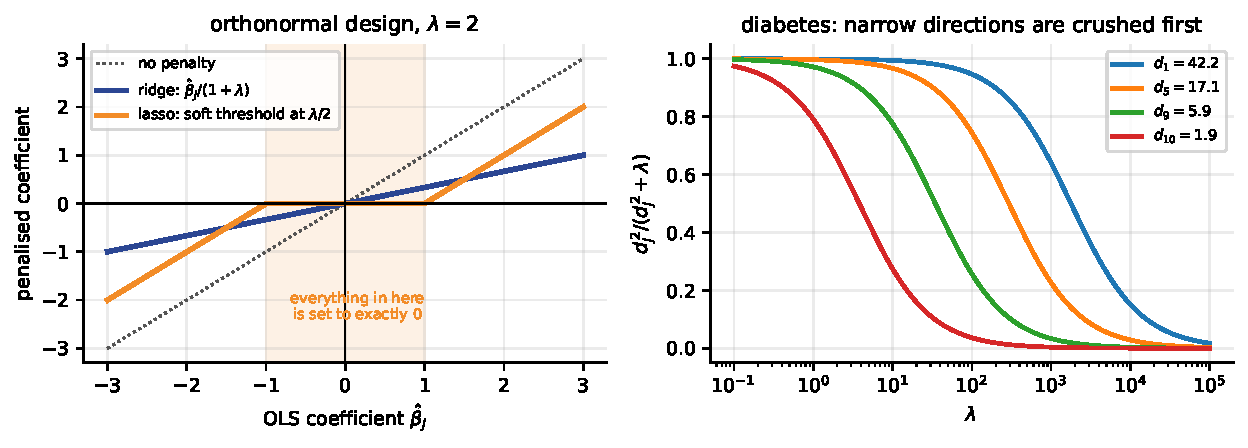
\includegraphics[width=0.95\textwidth]{shrinkage.pdf}
  \caption{Left: the two shrinkage rules on an orthonormal design at
  $\lambda = 2$. Ridge is a straight line through the origin of slope
  $1/(1+\lambda)$; it touches zero only at zero. Lasso is a line shifted
  towards the origin, with a flat dead zone of total width $\lambda$ in which
  every coefficient is set to exactly $0$. Right: on the standardised diabetes
  data, the shrinkage factor $d_j^2/(d_j^2 + \lambda)$ for four of the ten
  principal directions.}
  \label{fig:shrinkage}
\end{figure}

\subsection{No formula, so an algorithm: coordinate descent}
\label{sec:cd}

The general lasso is solved by \textbf{coordinate descent}: hold every
coefficient but one fixed, solve that one exactly --- which is the
one-dimensional problem of Section~\ref{sec:soft} --- and cycle until nothing
moves. Because the objective is convex and the non-smooth part is separable,
this converges to the global optimum.

\begin{lstlisting}
def soft_threshold(z, g):
    return np.sign(z) * max(abs(z) - g, 0.0)

def lasso_cd(X, y, alpha, iters=500):     # (1/2n)||y - Xb||^2 + alpha*||b||_1
    n, p = X.shape;  b = np.zeros(p);  r = y - X @ b
    norms = (X ** 2).sum(axis=0)
    for _ in range(iters):
        for j in range(p):
            r += X[:, j] * b[j]                       # take column j out
            rho = X[:, j] @ r / n
            b[j] = soft_threshold(rho, alpha) / (norms[j] / n)
            r -= X[:, j] * b[j]                       # put it back
    return b
\end{lstlisting}
\begin{codeout}
  alpha 0.5  my 20-line coordinate descent vs sklearn:  max |difference| 1.79e-10
     mine    [ 0.     -10.2874  24.9854  14.6692  -7.7751  0.      -8.4322   3.3024  24.9551   2.9069]
     sklearn [ 0.     -10.2874  24.9854  14.6692  -7.7751  0.      -8.4322   3.3024  24.9551   2.9069]
     exact zeros: mine 2, sklearn 2
  alpha 2.0  my 20-line coordinate descent vs sklearn:  max |difference| 9.29e-12
     mine    [ 0.      -7.5682  24.6228  13.1778  -2.7169  0.     -10.0536   0.      23.1479   1.6904]
     sklearn [ 0.      -7.5682  24.6228  13.1778  -2.7169  0.     -10.0536   0.      23.1479   1.6904]
     exact zeros: mine 3, sklearn 3
  the zeros are exact because the update ASSIGNS 0, it does not
  approach it. That is the whole difference from ridge.
\end{codeout}

Twenty lines reproduce \texttt{sklearn.linear\_model.Lasso} to eleven decimal
places. And the last sentence of that output is the point: the update
\emph{assigns} zero. It does not converge towards zero, so there is no
tolerance below which you have to decide whether something counts as zero.
That is why \texttt{(np.abs(coef) > 0).sum()} is a meaningful question for the
lasso and a silly one for ridge.

\subsection{The geometry: corners on the axes}
\label{sec:geometry}

Use the constrained form. The RSS is a quadratic in $\beta$, so its contours
are concentric ellipses centred on $\bhat^{\mathrm{OLS}}$ (their shape is set
by $\XtX$: circular if the columns are orthogonal, elongated and tilted if
they are correlated). The constrained solution is the point where the smallest
of those ellipses first \emph{touches} the feasible region.

In two dimensions, $\|\beta\|_1 \le t$ is a diamond with vertices at
$(\pm t, 0)$ and $(0, \pm t)$; $\|\beta\|_2 \le s$ is a disc of radius $s$.

\begin{keyidea}
The diamond's corners lie \emph{on the coordinate axes}, and at a corner all
but one coefficient is exactly zero. A corner is a point where the boundary
has no tangent, so an ellipse expanding from a generic centre is very likely
to strike a corner before it strikes any smooth part of the boundary. The disc
has no corners at all, so the touching point is generically in the interior of
a quadrant and every coefficient is non-zero.
\end{keyidea}

In $p$ dimensions the L1 ball is a cross-polytope with flat faces of every
dimension from $0$ (vertices, one non-zero coefficient) to $p-1$ (facets, all
non-zero): a whole hierarchy of ways to be sparse, and the ellipse picks one.
The L2 ball is a sphere, smooth everywhere.

\begin{codeout}
two features only, bmi and s4, standardised, y centred
  OLS         beta = [37.9402, 17.4475]   ||beta||_1 = 55.3876  ||beta||_2 = 41.7597
  the smallest lasso alpha that produces an exact zero is 24.7000
  lasso       beta = [20.4600, 0.0000]   ||beta||_1 = 20.4600  (budget t)
  ridge tuned to the SAME L1 budget (alpha = 1066.78):
  ridge       beta = [12.2323, 8.2277]   ||beta||_1 = 20.4600
  same budget, and lasso puts s4 at exactly 0 while ridge keeps it at 8.2277.
  RSS at OLS 1608070.9, at the lasso corner 1989017.7, at the ridge point 2024225.5
\end{codeout}

\begin{sloppypar}
Given \emph{the same} budget $\|\beta\|_1 \le 20.46$, the lasso answers
$(20.46,\ 0)$ while ridge answers $(12.23,\ 8.23)$.
\end{sloppypar}
Note also that the lasso's
corner has the \emph{lower} RSS of the two ($1{,}989{,}018$ against
$2{,}024{,}226$): under an L1 budget, spending everything on one predictor was
the better use of the money.

\begin{figure}[htbp]
  \centering
  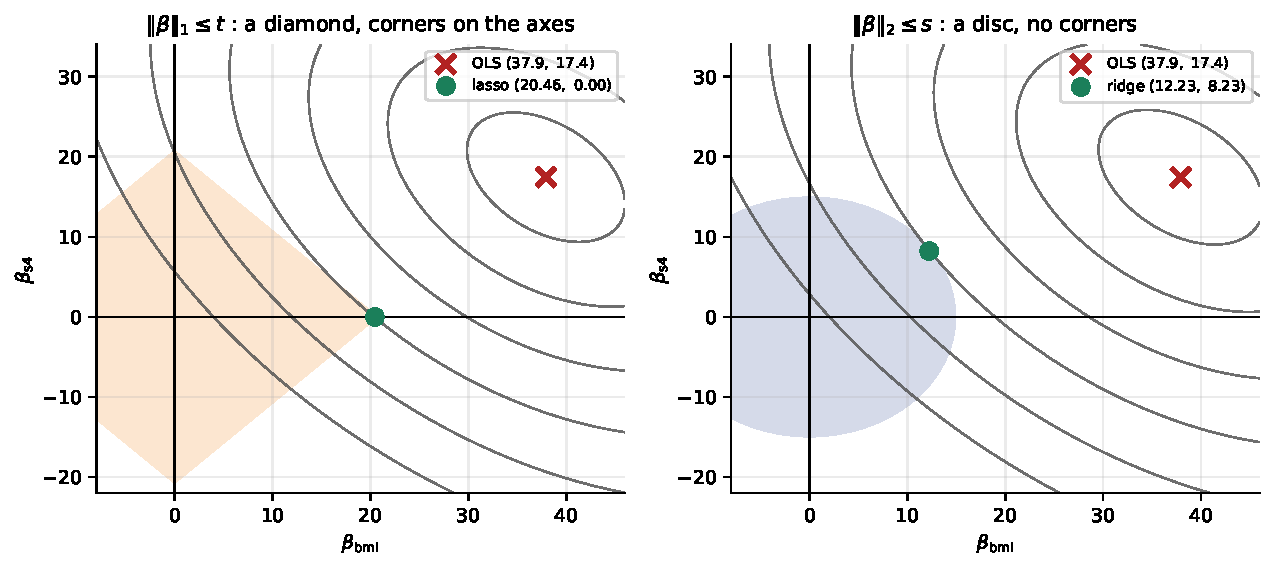
\includegraphics[width=0.95\textwidth]{geometry.pdf}
  \caption{Two standardised diabetes columns, \texttt{bmi} and \texttt{s4}.
  The grey curves are RSS contours centred on the OLS solution
  $(37.9, 17.4)$, tilted because the two columns correlate at $0.41$. Left:
  the L1 diamond; the smallest contour that reaches it does so at the corner,
  where $\beta_{\mathrm{s4}} = 0$ exactly. Right: the L2 disc scaled to the
  same L1 budget; the contour touches a smooth part of the boundary and both
  coefficients survive.}
  \label{fig:geometry}
\end{figure}

% =========================================================================
\section{Coefficient paths}
\label{sec:paths}

A \textbf{coefficient path} is the plot of every $\bhat_j$ against $\lambda$.
It is the single most informative picture in this lecture, because it shows
the whole family of models at once instead of one arbitrary member of it.

\begin{codeout}
diabetes, standardised, 10 features, alpha in sklearn units
  alpha        ridge nonzero  min|coef|   lasso nonzero  kept
  ridge a=0.01    lasso a=0.000    10        0.4756      10   age, sex, bmi, bp, s1, s2, s3, s4, s5, s6
  ridge a=1.00    lasso a=0.010    10        0.4312      10   age, sex, bmi, bp, s1, s2, s3, s4, s5, s6
  ridge a=10.00   lasso a=0.100    10        0.2579       9   age, sex, bmi, bp, s1, s2, s4, s5, s6
  ridge a=50.00   lasso a=0.500    10        0.1070       8   sex, bmi, bp, s1, s3, s4, s5, s6
  ridge a=100.00  lasso a=1.000    10        0.4361       7   sex, bmi, bp, s1, s3, s5, s6
ridge never returns an exact zero: smallest |coef| over the whole grid
   1.455e-03 at alpha up to 1e6 -- small, never 0
\end{codeout}

The ridge column reads ten, ten, ten, ten, ten. Sweeping $\alpha$ up to
$10^{6}$, where the coefficients are of order $10^{-3}$, still produces no
zero.

\begin{figure}[htbp]
  \centering
  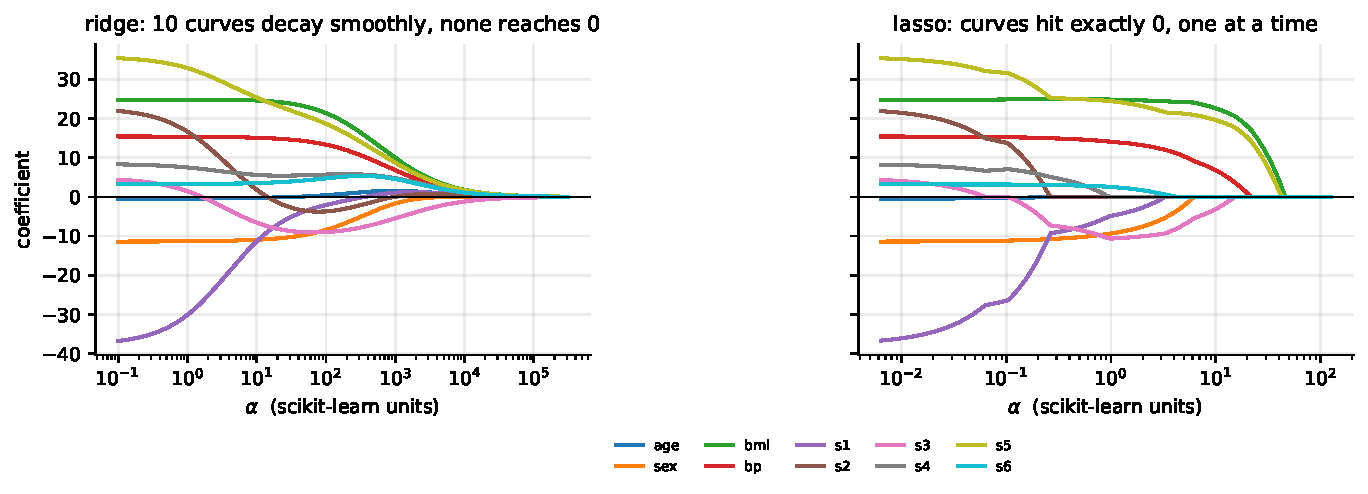
\includegraphics[width=\textwidth]{paths.pdf}
  \caption{The figure this lecture exists for. Ten standardised diabetes
  coefficients, one colour each, as $\alpha$ sweeps six orders of magnitude.
  Left, ridge: ten curves glide towards the axis and never arrive. Right,
  lasso: they land on it, one at a time, and stay there.}
  \label{fig:paths}
\end{figure}

\begin{codeout}
as alpha RISES, lasso coefficients hit exactly zero in this order:
    1. age  leaves at alpha =  0.2473
    2. s2   leaves at alpha =  0.2641
    3. s4   leaves at alpha =  0.9790
    4. s1   leaves at alpha =  3.2897
    5. s6   leaves at alpha =  4.2753
    6. sex  leaves at alpha =  6.3339
    7. s3   leaves at alpha = 15.3382
    8. bmi  leaves at alpha =     inf
    9. bp   leaves at alpha =     inf
   10. s5   leaves at alpha =     inf
number of non-zero coefficients along the path:
   alpha   5.00   nonzero  5   R2 on the training rows +0.4892
   alpha   1.00   nonzero  7   R2 on the training rows +0.5133
   alpha   0.05   nonzero 10   R2 on the training rows +0.5176
\end{codeout}

The order of departure is a ranking of the predictors, produced by the model
rather than by a univariate filter, and it accounts for the other variables at
every step. Half the features retain $94.5\%$ of the training $R^2$. The last
three standing --- body mass index, blood pressure and \texttt{s5} --- are the
three a clinician would have nominated.

\begin{caution}[The number of non-zero coefficients is not monotone]
It is tempting to assume that raising $\alpha$ can only remove features. It
usually does, but not always:
\begin{codeout}
   alpha  0.30  nonzero  8   coefficient on s3 -7.44693
   alpha  0.20  nonzero 10   coefficient on s3 -4.45426
   alpha  0.15  nonzero 10   coefficient on s3 -2.13916
   alpha  0.10  nonzero  9   coefficient on s3 -0.00000
   alpha  0.05  nonzero 10   coefficient on s3 +0.95082
   alpha  0.01  nonzero 10   coefficient on s3 +4.03508
\end{codeout}
The coefficient on \texttt{s3} travels from $+4.04$ to $-7.45$ as $\alpha$
rises, and passes through exactly zero near $\alpha = 0.10$ before leaving
again on the other side. It is a real feature of lasso paths, not a solver
bug, and it is why you should read a path rather than a single count.
\end{caution}

\begin{tryit}[Draw a path yourself]
Reproduce the right-hand panel of Figure~\ref{fig:paths} in about eight lines:
\begin{lstlisting}
X = StandardScaler().fit_transform(load_diabetes().data)
y = load_diabetes().target
al = np.logspace(-2.2, 2.1, 160)
C = np.array([Lasso(alpha=a, max_iter=200000).fit(X, y).coef_ for a in al])
plt.semilogx(al, C);  plt.axhline(0, color="k")
print((np.abs(C[np.abs(al - 5.0).argmin()]) > 1e-10).sum())
\end{lstlisting}
The last line should print \texttt{5}. Then change \texttt{Lasso} to
\texttt{Ridge} and print the same count: it will be \texttt{10} at every
$\alpha$ you try.
\end{tryit}

% =========================================================================
\section{Scaling is not optional}
\label{sec:scale}

\subsection{The argument}

The penalty $\lambda\sum_j\beta_j^2$ adds up $p$ numbers as though they were
commensurable. They are not, because a coefficient carries the reciprocal of
its predictor's unit.

Suppose you multiply column $j$ by a constant $c$. Under ordinary least
squares, $\bhat_j$ becomes $\bhat_j/c$, no other coefficient moves, and
\emph{every prediction is unchanged}: least squares is
\textbf{equivariant} under rescaling. Under ridge, $\bhat_j$ still wants to be
$\bhat_j/c$, but its contribution to the penalty is then
$\lambda\bhat_j^2/c^2$ --- different by a factor of $c^2$. So the optimum
moves.

\begin{keyidea}
A predictor recorded in \emph{large} numbers needs a \emph{small} coefficient,
pays almost no penalty, and is effectively unregularised. A predictor recorded
in \emph{small} numbers needs a \emph{large} coefficient, pays an enormous
penalty, and gets crushed. \textbf{The strength of the penalty on a variable
is decided by the unit somebody chose to record it in.}
\end{keyidea}

\subsection{Measured: where the budget goes}
\label{sec:budget}

Ridge with $\alpha = 100$ on the diabetes data in its original clinical units.

\begin{codeout}
raw-unit diabetes, 70/30 split. Ridge with alpha = 100.
  where the penalty budget goes when the columns keep their own units
     name    column sd    ridge coef   lambda*coef^2   share of penalty
     age       13.295       -0.1608            2.59         0.0002
     sex        0.500       -7.2829         5304.01         0.3758
     bmi        4.480        6.7139         4507.62         0.3194
     bp        13.846        0.9030           81.55         0.0058
     s1        34.433        1.3138          172.62         0.0122
     s2        30.394       -1.4654          214.75         0.0152
     s3        13.096       -2.3549          554.58         0.0393
     s4         1.325       -0.3681           13.55         0.0010
     s5         0.539        5.7095         3259.84         0.2310
     s6        12.321        0.1567            2.46         0.0002
\end{codeout}

The three narrowest columns --- \texttt{sex} ($\mathrm{sd}\ 0.50$),
\texttt{bmi} ($4.48$) and \texttt{s5} ($0.54$) --- consume
$0.3758 + 0.3194 + 0.2310 = 0.9262$ of the entire penalty budget.
\texttt{age} and \texttt{s6}, whose standard deviations are around $13$, pay
$0.0002$ each. The penalty is being spent on the columns with the smallest
numbers, not on the columns with the weakest evidence.

\subsection{Measured: one change of unit}
\label{sec:unit}

Divide \texttt{bmi} by $100$ --- report it as a fraction rather than in
kilograms per square metre. The information content is identical.

\begin{lstlisting}
Xtr2 = Xtr.copy();  Xtr2[:, 2] /= 100.0        # bmi, and nothing else
LinearRegression().fit(Xtr2, ytr);  Ridge(alpha=100.0).fit(Xtr2, ytr)
\end{lstlisting}
\begin{codeout}
     OLS   coef on bmi       6.2458 ->     624.5825   ratio   100.0000
     OLS   test R2     +0.392899 -> +0.392899   (the same fit)
     ridge coef on bmi       6.7139 ->       2.8018   ratio     0.4173
     ridge test R2     +0.358505 -> +0.309806   (a DIFFERENT model)
     bmi's share of the ridge penalty  0.3194 -> 0.0410
     max |prediction difference|, OLS   8.697e-12
     max |prediction difference|, ridge 71.0177
\end{codeout}

Under OLS the coefficient scaled by exactly $100$, the test $R^2$ agreed to
six decimal places, and the largest prediction difference over the whole test
set was $8.7\times10^{-12}$ --- floating-point noise. Under ridge, the
coefficient did \emph{not} scale by $100$ (the ratio is $0.42$), the test
$R^2$ fell by $0.049$, and predictions for the same patients moved by up to
$\mathbf{71.0}$ on a target that ranges from $25$ to $346$.

Under the lasso the effect is even less subtle, because the lasso deletes.

\begin{codeout}
  the same unit change under lasso, which also selects:
     alpha 1  kg/m^2 units: kept 9  age sex bmi bp s1 s2 s3 s5 s6
     alpha 1  bmi/100    : kept 7  age sex bp s2 s3 s5 s6
     alpha 3  kg/m^2 units: kept 8  age sex bmi bp s1 s2 s3 s6
     alpha 3  bmi/100    : kept 7  age sex bp s1 s2 s3 s6
\end{codeout}

\texttt{bmi} --- the single most predictive variable in the dataset --- was
removed from the model, not because the evidence changed but because somebody
divided it by a hundred. \texttt{s1} went with it.

\begin{codeout}
  ridge across a grid of alpha, raw units against standardised:
        alpha     raw test R2   standardised test R2
              1      +0.3919            +0.3916
            100      +0.3585            +0.4073
           1000      +0.3570            +0.2924
          10000      +0.3539            +0.0699
         100000      +0.2301            +0.0081
        1000000      +0.0644            +0.0008
\end{codeout}

Standardised, the best available $\alpha$ reaches $0.4073$. On raw units the
curve never exceeds $0.3919$, and it achieves that only by turning the penalty
essentially off.

\begin{figure}[htbp]
  \centering
  
\includegraphics[width=\textwidth]{scaling.pdf}
  \caption{Left: the share of $\sum_j\beta_j^2$ each column consumes at
  $\alpha = 100$, raw units against standardised. Right: test $R^2$ against
  $\alpha$ for both. The orange curve is not a worse version of the purple
  one --- it is a different experiment, in which $\alpha$ means something
  else.}
  \label{fig:scaling}
\end{figure}

\begin{tryit}[The one-line habit]
Never write a bare estimator. Write
\begin{lstlisting}
pipe = make_pipeline(StandardScaler(), Ridge(alpha=100.0))
\end{lstlisting}
so the scaler is refitted inside every cross-validation fold. Confirm on the
diabetes data that \texttt{pipe.fit(Xtr, ytr).score(Xte, yte)} gives
\texttt{+0.4073} while \texttt{Ridge(alpha=100).fit(Xtr, ytr).score(Xte, yte)}
on the raw columns gives \texttt{+0.3585}.
\end{tryit}

\subsection{The intercept is not penalised}
\label{sec:intercept}

Shift every target upwards by $500$ and refit.

\begin{lstlisting}
m0 = Ridge(alpha=100.0).fit(Xc, ytr)
m1 = Ridge(alpha=100.0).fit(Xc, ytr + 500.0)
\end{lstlisting}
\begin{codeout}
ridge with alpha = 100, then the same fit with y shifted up by 500
  intercept       152.1197 ->     652.1197   difference 500.0000
  max |coefficient difference|  1.288e-14
  mean of y = 152.1197, intercept of the unshifted fit = 152.1197
\end{codeout}

The intercept absorbed the shift exactly and no coefficient moved by more than
$1.3\times10^{-14}$. That is what ``not penalised'' buys you: the model's
answer does not depend on where you put the zero of your measuring scale. Note
too that with centred predictors the intercept \emph{equals} $\bar y$.

What if you penalise it anyway? \texttt{fit\_intercept=False} on data whose
target averages $152$ forces the fitted surface through the origin.

\begin{codeout}
what happens if you DO penalise it -- fit_intercept=False on
uncentred y (the mean of y is 152.1, nowhere near zero):
   alpha        1   with intercept R2 +0.3916   without -3.8362
   alpha      100   with intercept R2 +0.4073   without -3.8990
   alpha    10000   with intercept R2 +0.0699   without -4.4512
as alpha -> infinity the penalised model must predict a constant.
That constant should be ybar = 152.1197, and it is:
   Ridge(alpha=1e12): intercept 152.1197, max|coef| 1.512e-08, prediction 152.1197
\end{codeout}

\begin{caution}[$R^2 = -3.84$]
Negative $R^2$ means worse than predicting the mean, and by a factor of nearly
five. Use \texttt{fit\_intercept=False} only when you have centred $y$
yourself, and check that you have.
\end{caution}

The last two lines are the sanity check on the whole framework: as
$\lambda \to \infty$ every coefficient is crushed and the model must predict a
constant. The right constant is $\bar y$, and the fit at
\texttt{alpha=1e12} returns exactly that.

% =========================================================================
\section{Choosing $\lambda$}
\label{sec:cv}

\subsection{The procedure}

\begin{enumerate}[leftmargin=*]
  \item Hold out a test set and do not look at it until the very end.
  \item On the training rows, take a \emph{logarithmic} grid of $\lambda$ ---
    logarithmic because $\lambda$ acts multiplicatively; a linear grid wastes
    almost all its points in a region where nothing changes.
  \item For each $\lambda$, run $k$-fold cross-validation and record the mean
    validation error \textbf{and its standard error across the folds}.
  \item Choose a $\lambda$ (two rules below), refit on all the training rows
    at that $\lambda$, and score once on the test set.
\end{enumerate}

\textbf{The minimum rule.} Take the $\lambda$ with the lowest mean CV error.

\textbf{The one-standard-error rule.} Compute
$\mathrm{SE} = \mathrm{sd}(\text{fold errors})/\sqrt{k}$ at the minimum, and
take the \emph{largest} $\lambda$ whose mean CV error is still below
$\text{minimum} + \mathrm{SE}$. The justification: the curve is nearly flat
near its bottom and each point on it is estimated with noise, so many
$\lambda$ are statistically indistinguishable from the best. Among
indistinguishable models, prefer the simpler one.

\subsection{Measured on the diabetes data}

\begin{lstlisting}
for a in alphas:
    s = -cross_val_score(Ridge(alpha=a), Ztr, ytr, cv=KFold(5, shuffle=True,
        random_state=0), scoring="neg_mean_squared_error")
    means.append(s.mean());  ses.append(s.std(ddof=1) / np.sqrt(len(s)))
\end{lstlisting}
\begin{codeout}
RIDGE, 5-fold CV on the training rows, 60 alphas from 1e-2 to 1e4
  minimum        alpha   22.6951   CV MSE  3050.64   se 219.00
  1-SE threshold                    CV MSE  3269.64
  1-SE choice    alpha  147.7378   CV MSE  3213.05
     alpha   22.6951  test R2 +0.3971  test MSE  3075.84  ||beta||   41.799
     alpha  147.7378  test R2 +0.4049  test MSE  3035.86  ||beta||   32.073
  for comparison, OLS (alpha = 0): test R2 +0.3929  test MSE  3097.12
  and the flat end of the curve, alpha = 1e4: CV MSE  5910.73
LASSO, same folds, 60 alphas from 1e-3 to ~16
  minimum        alpha    0.9769   CV MSE  3051.35   se 218.35
  1-SE choice    alpha    9.6926   CV MSE  3237.26
     alpha    0.9769  test R2 +0.3889  nonzero  8  age, sex, bmi, bp, s1, s3, s5, s6
     alpha    9.6926  test R2 +0.3616  nonzero  4  bmi, bp, s3, s5
sklearn's own searchers agree:
  RidgeCV.alpha_ = 28.6832   test R2 +0.3989
  LassoCV.alpha_ = 0.9769   test R2 +0.3889   nonzero 8
\end{codeout}

Several things to read here.

The 1-SE choice was the \emph{better} choice for ridge on this split:
$\alpha = 147.7$ scored $0.4049$ on the test set against $0.3971$ for the
CV minimum, with a coefficient vector $23\%$ shorter. Both beat OLS
($0.3929$). That is not guaranteed --- it is one split --- but it illustrates
why the flat region deserves respect.

For the lasso, the 1-SE choice cost $0.027$ of test $R^2$ and bought a model
with four features instead of eight. Whether that is a good trade depends on
what the model is for.

And \texttt{RidgeCV} chose $28.7$ where the hand-rolled loop chose $22.7$,
because \texttt{RidgeCV} searched a slightly different grid. The test scores
differ by $0.0018$. The lesson is that the exact $\alpha$ is not the point;
the region is.

\begin{figure}[htbp]
  \centering
  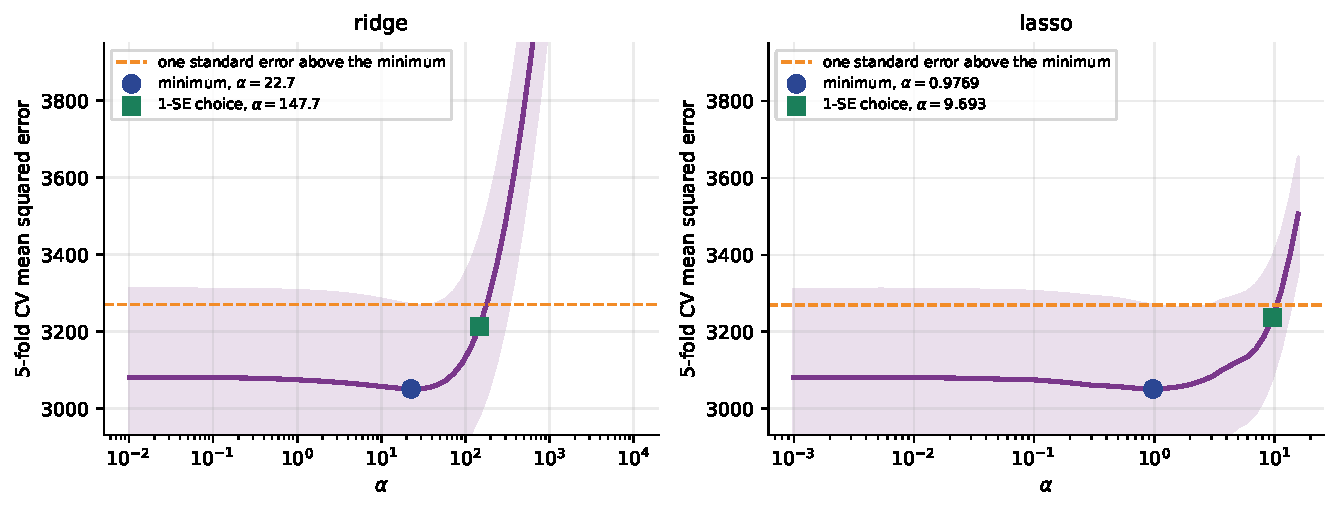
\includegraphics[width=\textwidth]{cvcurve.pdf}
  \caption{The validation curve for each penalty. The shaded band is
  $\pm$ one standard error across the five folds. Both curves are flat for
  three orders of magnitude and then climb steeply --- there is no sharp
  optimum to find. The dashed line is the 1-SE threshold and the square marks
  the largest $\alpha$ still beneath it.}
  \label{fig:cvcurve}
\end{figure}

\begin{caution}[The test set is scored once]
Choosing $\lambda$ by looking at the test score, and then reporting that
score, is the leakage of Unit IV wearing a new hat. $\lambda$ is chosen on
the training rows, by cross-validation, inside a \texttt{Pipeline}.
\end{caution}

% =========================================================================
\section{The trade being made: bias against variance}
\label{sec:bv}

\subsection{The algebra, where it is clean}

Ridge is a \textbf{biased} estimator, deliberately. Take $\XtX = I$ again so
that $\bhat^{R} = \bhat^{\mathrm{OLS}}/(1+\lambda)$, and recall that OLS is
unbiased with $\operatorname{Var}(\bhat^{\mathrm{OLS}}) = \sigma^2 I$. Then
\[
  \mathbb{E}[\bhat^{R}] = \frac{\beta}{1+\lambda},
  \qquad
  \operatorname{bias}(\bhat^{R}) = -\frac{\lambda}{1+\lambda}\,\beta,
  \qquad
  \operatorname{Var}(\bhat^{R}) = \frac{\sigma^2}{(1+\lambda)^2}\,I .
\]
Summing squared bias and variance over the $p$ coordinates,
\begin{equation}
  \mathrm{MSE}(\lambda)
  = \underbrace{\frac{\lambda^2\|\beta\|^2}{(1+\lambda)^2}}_{\text{bias}^2,
    \text{ increasing}}
  + \underbrace{\frac{\sigma^2 p}{(1+\lambda)^2}}_{\text{variance},
    \text{ decreasing}}
  = \frac{\lambda^2\|\beta\|^2 + \sigma^2 p}{(1+\lambda)^2} .
  \label{eq:mse}
\end{equation}

Differentiate. Writing $B = \|\beta\|^2$,
\[
  \mathrm{MSE}'(\lambda)
  = \frac{2\lambda B (1+\lambda)^2 - 2(1+\lambda)(\lambda^2 B + \sigma^2 p)}
         {(1+\lambda)^4}
  = \frac{2\big(\lambda B - \sigma^2 p\big)}{(1+\lambda)^3} .
\]

\begin{keyidea}
The minimum is at $\lambda^\star = \sigma^2 p / \|\beta\|^2$, and
$\mathrm{MSE}'(0) = -2\sigma^2 p < 0$. \textbf{$\lambda = 0$ is never optimal.}
There is always a strictly positive $\lambda$ whose ridge estimator has lower
expected squared error than ordinary least squares. This is the
Hoerl--Kennard result, and it is why regularization is not a heuristic.
\end{keyidea}

The formula also tells you \emph{how much} penalty: a lot when the noise
$\sigma^2$ is large, a lot when there are many parameters $p$, and little when
the true signal $\|\beta\|^2$ is strong.

\subsection{Measured, on 400 training sets}

Fix a test set of $500$ points. Draw a fresh training set of $n = 40$ from the
same generator, $400$ times over; fit ridge at each $\lambda$; and decompose
the average squared error at each test point into
$(\text{mean prediction} - \text{truth})^2$ and the variance of the
predictions.

\begin{lstlisting}
rng = np.random.default_rng(0)              # the one seed for this lecture
for r in range(400):
    Xt = rng.normal(size=(40, 25))
    yt = Xt @ beta + rng.normal(0, 2.0, 40)
    for i, lam in enumerate(lams):
        preds[i, r] = Ridge(alpha=lam, fit_intercept=False).fit(Xt, yt).predict(Xte)
bias2 = ((preds.mean(axis=1) - f_true) ** 2).mean(axis=1)
var   = preds.var(axis=1).mean(axis=1)
\end{lstlisting}
\begin{codeout}
simulation: p = 25, n = 40, sigma = 2.0, 400 training sets, 500 fixed test points
  lambda      bias^2   variance   noise   expected test MSE
      0.010    0.0226     6.9702    4.00     10.9928
      0.134    0.0199     6.6164    4.00     10.6363
      1.805    0.1585     4.3535    4.00      8.5119
      4.781    0.6766     3.1703    4.00      7.8469
    170.125   12.1011     0.3214    4.00     16.4225
   3162.278   17.2243     0.0022    4.00     21.2265
  minimum of the total at lambda = 4.781
  at lambda -> 0   : bias^2 0.0226  variance   6.9702  total   10.9928
  at the optimum   : bias^2 0.6766  variance   3.1703  total    7.8469
  variance removed 3.7998, bias added 0.6540, net gain 3.1459
  the net gain is 45.0% of the reducible error (10.9928 - 4.00 = 6.9928)
  check: bias^2 + variance reproduces the measured squared error to 7.11e-15
  orthonormal-design theory says the best lambda is sigma^2 p / ||beta||^2 = 5.4298
  ||beta||^2 = 18.4169
  measured optimum 4.781 -- the same order, 14% high; X'X here is Wishart, not I.
\end{codeout}

At the optimum, $0.65$ of bias$^2$ was added and $3.80$ of variance was
removed: a net saving of $\mathbf{3.15}$, which is $45\%$ of the reducible
error ($10.99 - 4.00 = 6.99$). The decomposition reproduces the directly
measured squared error to $7\times10^{-15}$, so the identity
\[
  \mathbb{E}\big[(\hat f(x) - f(x))^2\big]
  = \big(\mathbb{E}\hat f(x) - f(x)\big)^2 + \operatorname{Var}\hat f(x)
\]
is not an approximation.

And the closed form of Equation~\eqref{eq:mse} landed in the right place
without being exact: $\sigma^2 p/\|\beta\|^2 = 5.43$ against a measured
$4.78$, some $14\%$ high. It is not exact here because $\XtX$ for a random
Gaussian design is Wishart, not the identity --- but it is the right order of
magnitude, and it tells you what to try first.

\begin{figure}[htbp]
  \centering
  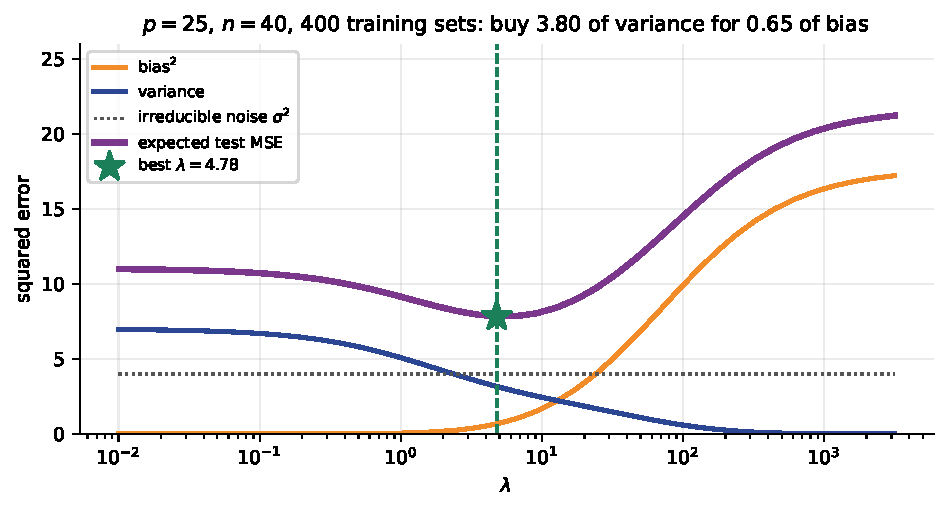
\includegraphics[width=0.82\textwidth]{biasvar.pdf}
  \caption{Bias$^2$ climbing from nothing, variance falling to nothing, and
  their sum with a minimum strictly to the right of zero. The dotted line is
  $\sigma^2 = 4$, the part no estimator can remove. The far left of the purple
  curve is ordinary least squares; the far right is the constant model.}
  \label{fig:biasvar}
\end{figure}

% =========================================================================
\section{Elastic net}
\label{sec:enet}

\subsection{Both penalties at once}

\begin{equation}
  \text{RSS} \;+\; \lambda\Big[\,\rho\sum_j|\beta_j|
    \;+\; (1-\rho)\sum_j\beta_j^2\,\Big],
  \qquad \rho \in [0, 1] .
  \label{eq:enet}
\end{equation}

In scikit-learn this is \texttt{ElasticNet(alpha=$\lambda$,
l1\_ratio=$\rho$)}; $\rho = 1$ is the lasso and $\rho = 0$ is ridge.

It exists to fix a specific failure. Given a group of strongly correlated
predictors that all carry the same signal, the lasso will keep one of them and
discard the rest --- and \emph{which} one it keeps is close to arbitrary. The
L2 term repairs this, because $\sum_j\beta_j^2$ is minimised, for a fixed
total, by spreading the weight evenly. So the L2 part wants the group to
share, while the L1 part still permits the whole group to be dropped together.
This is the \textbf{grouping effect}. A second benefit: when $p > n$, the
lasso can select at most $n$ variables; the elastic net has no such limit.

\subsection{Measured}

Three near-copies of one latent signal (pairwise correlation $0.9971$), plus
seven pure-noise columns.

\begin{codeout}
  lasso       coefficients on the group [2.1943 0.3251 0.0565]
  elastic net coefficients on the group [0.8844 0.8606 0.8602]
  ridge       coefficients on the group [0.806  0.7954 0.7973]
stability: refit on 30 bootstrap resamples and count how often each
of the three group members is kept.
  lasso       kept x1 29/30, x2 13/30, x3 21/30   median group size kept 2.0
  elastic net kept x1 30/30, x2 30/30, x3 30/30
prediction on 400 fresh rows, scaler fitted on the training rows only:
  lasso        test R2 +0.9609
  elastic net  test R2 +0.9636
  ridge        test R2 +0.9435
\end{codeout}

The three columns are statistically indistinguishable from each other, and
the lasso does not treat them that way. On the full sample it puts $2.19$ on
$x_1$ and almost nothing on the other two; resampled thirty times it keeps
$x_1$ in $29$ resamples, $x_3$ in $21$ and $x_2$ in only $13$. Nothing in the
data distinguishes those three columns; the ranking is an artefact of which
rows happened to be drawn. If you report ``the lasso selected $x_1$'', you are
reporting a coin flip. The elastic net keeps all three, every time.

\begin{keyidea}
A variable selection is a statistic, and like any statistic it has a sampling
distribution. Resample and refit; if the selected set changes, say so.
\textbf{Report a selection with its stability, or do not report it.}
\end{keyidea}

\begin{figure}[htbp]
  \centering
  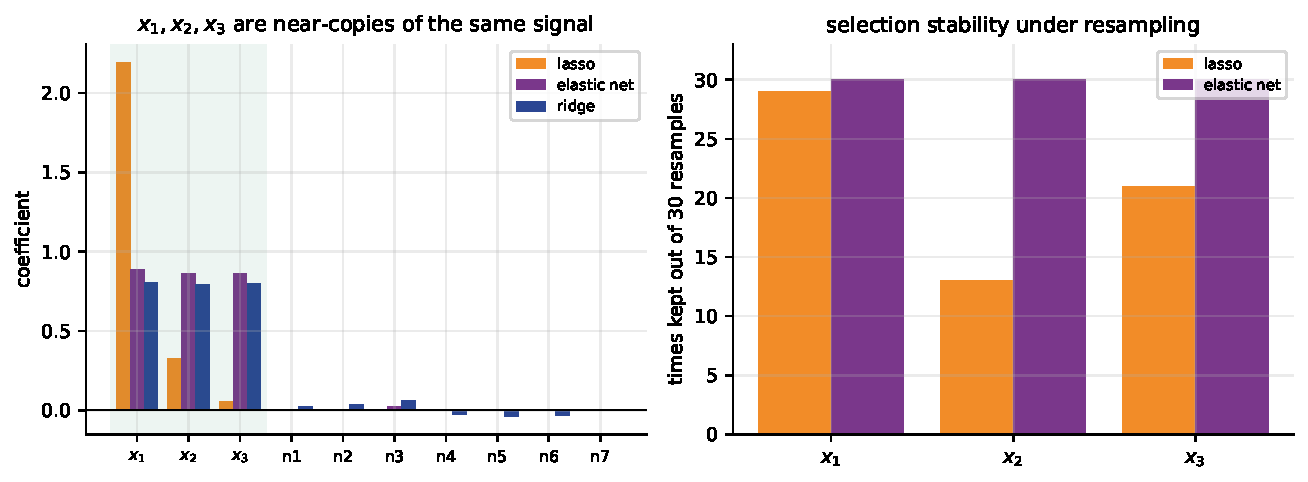
\includegraphics[width=\textwidth]{elasticnet.pdf}
  \caption{Left: the fitted coefficients. Lasso piles $2.19$ onto one member
  of the group and leaves $0.33$ and $0.06$ for the other two; elastic net and
  ridge spread roughly $0.87$ and $0.80$ evenly across all three. Right: how
  often each group member survived a bootstrap resample.}
  \label{fig:enet}
\end{figure}

\subsection{All four on the same data}

\begin{lstlisting}
pipe = make_pipeline(StandardScaler(), RidgeCV(alphas=np.logspace(-2, 4, 60),
                                               cv=KFold(5, shuffle=True,
                                                        random_state=0)))
pipe.fit(X_train, y_train);  pipe.score(X_test, y_test)
\end{lstlisting}
\begin{codeout}
diabetes, 70/30 split, everything inside a Pipeline
  model              train R2   test R2   nonzero of 10
  OLS                 +0.5539   +0.3929        10
  Ridge, CV alpha     +0.5505   +0.3989        10
  Lasso, CV alpha     +0.5517   +0.3889         8
  ElasticNet 0.5      +0.5529   +0.3917        10
\end{codeout}

\begin{caution}[Report this honestly]
On a $442\times10$ problem with no collinearity crisis, regularization is
worth about six thousandths of $R^2$, and lasso is very slightly worse than
OLS. That is the truthful result and you should say so. Its value here is not
accuracy: it is that the lasso answered the question ``which eight of the ten
do we need?''. Go back to the $n = 50$, $p = 100$ table in
Section~\ref{sec:pgtn} for the case where the same machinery lifts test
$R^2$ from $0.4183$ to $0.6303$ on one draw, and from a mean of $0.4446$ to a
mean of $0.6532$ across twenty --- the difference between a fit that barely
generalises and one that does.
\end{caution}

% =========================================================================
\section{Summary}

\begin{enumerate}[leftmargin=*]
  \item Regularization means minimising
    $\text{loss}(\beta) + \lambda\,\text{pen}(\beta)$. $\lambda$ is a
    hyper-parameter, chosen by cross-validation, never estimated by the fit.
  \item Ridge has the closed form
    $\bhat = (\XtX + \lambda I)^{-1}\Xty$, derived in four lines from
    $\nabla J = 0$, with $\lambda = 0$ recovering ordinary least squares.
  \item $\XtX + \lambda I$ is positive definite for every $\lambda > 0$,
    because $v^{\!\top}(\XtX + \lambda I)v = \|Xv\|^2 + \lambda\|v\|^2$.
    Equivalently, its eigenvalues are $d_j^2 + \lambda > 0$. \textbf{Ridge
    exists where OLS does not.} On $X$ with a column exactly twice another,
    $\det(\XtX) = 0$ and \texttt{np.linalg.inv} raises; $\lambda = 1$ makes
    the determinant $71$.
  \item At $p > n$, \texttt{LinearRegression} does not fail --- it silently
    returns the minimum-norm solution, which is exactly ridge at
    $\lambda \to 0$ (agreeing to $5.9\times10^{-12}$). ``OLS'' at $p>n$ is
    already a regularised estimator.
  \item By hand: $x = (1,2,2)$, $y = (2,3,5)$ gives
    $\bhat = 18/(9+\lambda)$, so $2.0 \to 1.8 \to 1.0 \to 0.2$ at
    $\lambda = 0, 1, 9, 81$; \texttt{Ridge} reproduces all four exactly. The
    $2\times2$ case gives $(1, 2) \to (0.875, 1.375) \to (0.625, 0.875)$.
  \item In the SVD basis ridge multiplies direction $j$ by
    $d_j^2/(d_j^2+\lambda)$, crushing the \emph{narrow} directions first. On
    diabetes, $\mathrm{df}(\lambda)$ falls from $10$ to $2.51$ at
    $\lambda = 1000$.
  \item The lasso has no closed form because $|\beta|$ has no derivative at
    $0$; the stationarity condition involves a subdifferential that cannot be
    inverted. On an orthonormal design it is soft thresholding, and
    $(3, 1, -0.4, 0.2)$ becomes $(2.5, 0.5, 0, 0)$ --- two exact zeros ---
    where ridge gives $(1.5, 0.5, -0.2, 0.1)$. Twenty lines of coordinate
    descent reproduce \texttt{Lasso} to $10^{-11}$.
  \item Geometrically the L1 ball is a diamond with corners \emph{on the
    axes} and the L2 ball is a smooth disc. At the same L1 budget of
    $20.46$, lasso answered $(20.46,\ 0)$ and ridge $(12.23,\ 8.23)$.
  \item Ridge sweeps never produce a zero (smallest coefficient
    $1.5\times10^{-3}$ at $\alpha = 10^{6}$); lasso sweeps delete features in
    a definite order, and half the diabetes features retain $94.5\%$ of the
    training $R^2$.
  \item Scaling is not optional. Three narrow raw columns took $92.6\%$ of the
    ridge penalty. Dividing \texttt{bmi} by $100$ moved OLS predictions by
    $8.7\times10^{-12}$ and ridge predictions by $71.0$, and made the lasso
    \textbf{delete \texttt{bmi} entirely}.
  \item The intercept is not penalised: shifting $y$ by $500$ moved the
    intercept by exactly $500.0000$ and no coefficient by more than
    $1.3\times10^{-14}$. Penalise it and test $R^2$ becomes $-3.84$. As
    $\lambda\to\infty$ the model predicts $\bar y$, and it does.
  \item Cross-validation gave ridge $\alpha = 22.7$ (test $R^2 = 0.3971$) and
    the 1-SE rule $\alpha = 147.7$ (test $R^2 = 0.4049$); the lasso's 1-SE
    choice kept four features of ten at a cost of $0.027$.
  \item The trade, measured: at $\lambda^\star = 4.78$, bias$^2$ rose by
    $0.65$ and variance fell by $3.80$, a net gain of $3.15$. The closed form
    $\lambda^\star = \sigma^2 p/\|\beta\|^2$ predicted $5.43$. And
    $\mathrm{MSE}'(0) < 0$ always: \textbf{$\lambda = 0$ is never optimal}.
  \item Elastic net exists for correlated groups. Of an indistinguishable
    trio the lasso kept one member in $29$ of $30$ resamples and another in
    only $13$; elastic net kept all three in $30$ of $30$, and predicted
    marginally better.
\end{enumerate}

% =========================================================================
\section{Practice questions}
\label{sec:practice}

Attempt these before reading Section~\ref{sec:solutions}. Questions 1--5 and 7
are pure hand work and are the ones most likely to appear on a paper.

\begin{enumerate}[leftmargin=*]
  \item\label{q:hand1} A single predictor takes the values
    $x = (2, 2, 4)$ and the target is $y = (3, 5, 8)$, with no intercept.
    (a) Compute $\XtX$ and $\Xty$. (b) Give $\bhat(\lambda)$ as a formula.
    (c) Evaluate it at $\lambda = 0$, $\lambda = 6$ and $\lambda = 24$, and
    state the shrinkage factor in each case. (d) At what $\lambda$ is the
    coefficient one third of its least-squares value?

  \item\label{q:hand2} A design has
    $\XtX = \left(\begin{smallmatrix}4&2\\2&4\end{smallmatrix}\right)$ and
    $\Xty = (6, 3)^{\!\top}$. (a) Find $\bhat^{\mathrm{OLS}}$ by hand.
    (b) Find $\bhat^{\mathrm{ridge}}$ at $\lambda = 2$ and at $\lambda = 8$.
    (c) Report $\|\bhat\|_2$ for all three and confirm it decreases.
    (d) Do both coefficients shrink by the same proportion? Explain.

  \item\label{q:sing} A design matrix has three columns, and the third is the
    sum of the first two. (a) What is $\operatorname{rank}(\XtX)$ at most, and
    what is $\det(\XtX)$? (b) What will \texttt{np.linalg.inv(X.T @ X)} do?
    (c) What will \texttt{LinearRegression().fit(X, y)} do, and why is that
    worse than raising an exception? (d) What is the smallest eigenvalue of
    $\XtX + 5I$?

  \item\label{q:proof} Prove that $\XtX + \lambda I$ is positive definite for
    every $\lambda > 0$ and every real $X$, and explain which step of the
    proof fails when $\lambda = 0$. Then state the consequence for the
    existence and uniqueness of the ridge estimator.

  \item\label{q:svd} A standardised design has singular values
    $d = (10, 5, 1)$. (a) Compute the shrinkage factor
    $d_j^2/(d_j^2+\lambda)$ for each direction at $\lambda = 25$.
    (b) Compute $\mathrm{df}(\lambda)$ at $\lambda = 25$. (c) Which direction
    is most affected, and what does that direction correspond to in the data?
    (d) What is $\mathrm{df}(0)$?

  \item\label{q:scale} You fit \texttt{Ridge(alpha=1.0)} to a table whose
    columns are a person's age in years, their annual income in rupees, and
    the number of children they have. (a) Rank the three columns by the
    fraction of the penalty each is likely to consume, and justify the
    ranking. (b) What happens to each coefficient if you switch the income
    column from rupees to lakhs? (c) What would happen under ordinary least
    squares instead? Quantify (b) and (c) using the measured numbers in
    Section~\ref{sec:unit}.

  \item\label{q:soft} On an orthonormal design the OLS coefficients are
    $(2.4,\ -1.1,\ 0.6,\ -0.3)$. (a) Give the ridge and lasso solutions at
    $\lambda = 1.2$ in the textbook parameterisation. (b) How many exact zeros
    does each produce? (c) What is the smallest $\lambda$ at which the lasso
    returns exactly two non-zero coefficients? (d) What is the smallest
    $\lambda$ at which ridge returns any zero at all?

  \item\label{q:geom} Explain, in your own words and without using the word
    ``corner'' more than once, why the lasso produces exact zeros and ridge
    does not. Give both the algebraic reason (from the derivative of the
    penalty) and the geometric reason. Then say what changes in three
    dimensions.

  \item\label{q:cv} A colleague reports: ``I fitted ridge with
    \texttt{alpha=1.0}, got test $R^2 = 0.42$, then tried
    \texttt{alpha=10}, got $0.44$, then \texttt{alpha=100}, got $0.46$, so I
    am reporting $0.46$.'' (a) Identify the methodological error.
    (b) Describe the correct procedure. (c) State the one-standard-error rule
    and give one reason to prefer it. (d) Using
    Section~\ref{sec:cv}, quantify how much difference the choice between the
    minimum and the 1-SE rule made on the diabetes data, for both penalties.

  \item\label{q:design} You are given a gene-expression table with $n = 60$
    patients and $p = 8000$ genes, and asked for (i) the best possible
    prediction and (ii) a shortlist of at most $30$ genes for a follow-up
    assay. Design the analysis. For each decision, cite a measured number from
    these notes. Say explicitly what you would do about scaling, about
    choosing $\lambda$, about the fact that $p \gg n$, and about reporting the
    shortlist.
\end{enumerate}

% =========================================================================
\section{Solutions}
\label{sec:solutions}

\textbf{1.} (a) $\XtX = 4 + 4 + 16 = 24$;
$\Xty = 2\cdot3 + 2\cdot5 + 4\cdot8 = 6 + 10 + 32 = 48$.

(b) $\bhat(\lambda) = 48/(24 + \lambda) = 2 \times 24/(24+\lambda)$.

(c) $\lambda = 0$: $\bhat = 2$, factor $1$. $\lambda = 6$:
$48/30 = 1.6$, factor $0.8$. $\lambda = 24$: $48/48 = 1$, factor
$0.5$ --- again the coefficient halves at $\lambda = \XtX$, as in
Section~\ref{sec:hand1}.

(d) Solve $24/(24+\lambda) = 1/3$, giving $24 + \lambda = 72$ and
$\lambda = 48 = 2\XtX$. In general the coefficient is a fraction $f$ of its
OLS value at $\lambda = \XtX(1-f)/f$.

\medskip
\textbf{2.} (a) $\det = 16 - 4 = 12$, so
\[
  \bhat^{\mathrm{OLS}} = \frac{1}{12}
  \begin{pmatrix}4 & -2\\ -2 & 4\end{pmatrix}
  \begin{pmatrix}6\\3\end{pmatrix}
  = \frac{1}{12}\begin{pmatrix}24 - 6\\ -12 + 12\end{pmatrix}
  = \begin{pmatrix}1.5\\0\end{pmatrix}.
\]

(b) At $\lambda = 2$: the matrix is
$\left(\begin{smallmatrix}6&2\\2&6\end{smallmatrix}\right)$, $\det = 32$,
\[
  \bhat = \tfrac{1}{32}\begin{pmatrix}6&-2\\-2&6\end{pmatrix}
  \begin{pmatrix}6\\3\end{pmatrix}
  = \tfrac{1}{32}\begin{pmatrix}30\\6\end{pmatrix}
  = (0.9375,\ 0.1875).
\]
At $\lambda = 8$: the matrix is
$\left(\begin{smallmatrix}12&2\\2&12\end{smallmatrix}\right)$, $\det = 140$,
$\bhat = \tfrac{1}{140}(72 - 6,\ -12 + 36) = (0.4714,\ 0.1714)$.

(c) $\|\bhat\|_2 = 1.5000$, $0.9561$, $0.5016$. Decreasing, as it must:
increasing $\lambda$ tightens the constraint $\|\beta\|_2 \le s$.

(d) No. $\beta_2$ started at exactly $0$ and became \emph{positive}. That is
not a failure of the arithmetic: ridge is
$(\XtX+\lambda I)^{-1}\Xty$, and changing the matrix changes the direction of
the solution, not just its length. Ridge is a uniform rescaling only when
$\XtX \propto I$, which this is not (the off-diagonal is $2$).

\medskip
\textbf{3.} (a) At most $2$, because the three columns span a
two-dimensional space; $\det(\XtX) = 0$ exactly, since a rank-deficient
matrix has a zero eigenvalue.

(b) It raises \texttt{numpy.linalg.LinAlgError: Singular matrix}, as in
Section~\ref{sec:singular}.

(c) It returns a coefficient vector without any warning. Internally it calls
\texttt{lstsq}, which selects the minimum-$\|\beta\|_2$ member of the infinite
solution set. That is worse than an exception because the output looks
ordinary: you will read and interpret coefficients that were chosen by a
tie-breaking rule you did not know was applied. The measured demonstration is
in Section~\ref{sec:pgtn}, where \texttt{lstsq} and ridge at
$\lambda = 10^{-9}$ agree to $5.9\times10^{-12}$.

(d) $5$. The eigenvalues of $\XtX + 5I$ are $d_j^2 + 5$, and the smallest
$d_j^2$ is $0$.

\medskip
\textbf{4.} Let $v \in \mathbb{R}^p$, $v \ne 0$. Then
\[
  v^{\!\top}(\XtX + \lambda I)v = v^{\!\top}\XtX v + \lambda v^{\!\top}v
  = (Xv)^{\!\top}(Xv) + \lambda v^{\!\top}v = \|Xv\|^2 + \lambda\|v\|^2 .
\]
Both terms are non-negative. The second is \emph{strictly} positive because
$\lambda > 0$ and $v \ne 0$, so the sum is strictly positive. A symmetric
matrix with this property is positive definite, hence all its eigenvalues are
strictly positive, hence $\det \ne 0$ and the inverse exists.

At $\lambda = 0$ the second term vanishes and the bound collapses to
$\|Xv\|^2 \ge 0$, which is not strictly positive: if $X$ has a non-trivial
null space there is a $v \ne 0$ with $Xv = 0$, and then
$v^{\!\top}\XtX v = 0$. So $\XtX$ is only positive \emph{semi}-definite in
general, and singular whenever the columns are linearly dependent --- which
includes every case with $p > n$.

Consequence: the ridge objective is strictly convex for $\lambda > 0$, so it
has exactly one minimiser and it is given by Equation~\eqref{eq:ridge}. The
least-squares objective is only convex, so its minimiser exists but need not
be unique.

\medskip
\textbf{5.} (a) $d_j^2 = (100, 25, 1)$, so the factors are
$100/125 = 0.8000$, $25/50 = 0.5000$, $1/26 = 0.0385$.

(b) $\mathrm{df}(25) = 0.8 + 0.5 + 0.0385 = 1.3385$.

(c) The third, which keeps under $4\%$ of itself. It is the direction along
which the data vary least --- the near-collinear combination of the original
columns. Along that direction the least-squares estimate has the largest
variance (its variance is proportional to $1/d_j^2$), so it is exactly the
estimate you should trust least, and ridge shrinks it most. This is the
alignment described in Section~\ref{sec:svd}.

(d) $\mathrm{df}(0) = 1 + 1 + 1 = 3 = p$: with no penalty, all three
directions are used in full.

\medskip
\textbf{6.} (a) Income will consume by far the least penalty; number of
children the most; age in between. A coefficient carries the reciprocal of its
predictor's unit, so a column whose numbers are in the hundreds of thousands
needs a coefficient of order $10^{-5}$, contributing about $10^{-10}$ to
$\sum\beta_j^2$. Number of children ranges over roughly $0$ to $5$, so its
coefficient must be of order of the target itself, and it dominates the sum.
Section~\ref{sec:budget} measures exactly this: three columns with standard
deviations of $0.50$, $4.48$ and $0.54$ took $92.6\%$ of the budget, while
columns with standard deviations around $13$ and $34$ took $0.02\%$ and
$1.2\%$.

(b) Switching from rupees to lakhs divides the numbers by $100{,}000$, so
under ridge the income coefficient must grow by roughly that factor, its
penalty contribution grows by roughly $10^{10}$, and the penalty crushes it.
The whole model changes: other coefficients move to compensate, and the
predictions change. Section~\ref{sec:unit} measures a factor of only $100$ on
one column and still finds predictions moving by $71.0$ units and the ridge
test $R^2$ falling from $0.3585$ to $0.3098$; under the lasso the rescaled
column was \emph{deleted}.

(c) Under OLS, nothing happens that matters: the income coefficient is
multiplied by exactly $100{,}000$, no other coefficient moves, and every
prediction is identical. Measured: the largest prediction difference over the
whole test set was $8.7\times10^{-12}$, which is floating-point noise. Least
squares is equivariant under rescaling; penalised least squares is not.

The fix in both cases is \texttt{make\_pipeline(StandardScaler(),
Ridge(...))}.

\medskip
\textbf{7.} (a) Threshold $\lambda/2 = 0.6$; ridge divisor
$1 + \lambda = 2.2$.
\begin{center}
\begin{tabular}{@{}lrrrr@{}}
\toprule
$\bhat_j$ & $2.4$ & $-1.1$ & $0.6$ & $-0.3$\\
\midrule
ridge $\bhat_j/2.2$ & $1.0909$ & $-0.5000$ & $0.2727$ & $-0.1364$\\
lasso, threshold $0.6$ & $1.8$ & $-0.5$ & $0$ & $0$\\
\bottomrule
\end{tabular}
\end{center}
Note $|0.6| = 0.6$ is exactly at the threshold, so it maps to $0$.

(b) Ridge: none. Lasso: two.

(c) The lasso keeps $\bhat_j$ iff $|\bhat_j| > \lambda/2$. Sorting the
magnitudes: $2.4, 1.1, 0.6, 0.3$. Exactly two survive when
$1.1 > \lambda/2 \ge 0.6$, that is $1.2 \le \lambda < 2.2$. The smallest such
$\lambda$ is $1.2$ --- which is the value in part (a), consistent with the
answer to (b).

(d) There is none. $\bhat_j/(1+\lambda)$ is zero only if $\bhat_j$ is zero,
for any finite $\lambda$. This is the measured claim of
Section~\ref{sec:paths}: the smallest ridge coefficient anywhere on a sweep to
$\alpha = 10^{6}$ was $1.455\times10^{-3}$.

\medskip
\textbf{8.} \emph{Algebraically.} The force a penalty exerts on a coefficient
is the derivative of the penalty. For L2 that force is $2\lambda\beta_j$,
which fades to nothing as the coefficient approaches the origin, so there is
never enough pull at the last step to complete the journey; the coefficient
asymptotes towards zero without arriving. For L1 the force is
$\lambda\operatorname{sign}(\beta_j)$, of constant magnitude no matter how
small the coefficient is. Once the residual correlation of a predictor drops
below that constant force, the optimum for that coefficient is at the origin
and it is pinned there.

\emph{Geometrically.} Solve the constrained version. The residual sum of
squares has elliptical contours around the least-squares point, and the
solution is where the innermost reachable ellipse touches the feasible set.
The L1 feasible set is a diamond whose vertices sit on the coordinate axes;
its boundary is not smooth at those points, so an expanding ellipse arriving
from a generic direction meets one of them first, and at such a point all but
one coefficient is exactly zero. The L2 feasible set is a disc, differentiable
at every boundary point, with no distinguished points for the ellipse to
catch on --- so the touching point falls in the interior of a quadrant and
every coefficient is non-zero. Figure~\ref{fig:geometry} shows both, on the
same data and at the same L1 budget: $(20.46, 0)$ against $(12.23, 8.23)$.

\emph{In three dimensions.} The L1 ball becomes an octahedron. It now has
faces of three kinds: six vertices (one non-zero coefficient), twelve edges
(two non-zero), and eight triangular facets (all three non-zero). An ellipsoid
can touch any of them, so the lasso can return any level of sparsity, with
sparser solutions favoured because the lower-dimensional features stick out
further relative to the smooth parts. The L2 ball becomes a sphere, still
smooth everywhere, still giving three non-zero coefficients. In $p$
dimensions the pattern continues to faces of every dimension from $0$ to
$p-1$.

\medskip
\textbf{9.} (a) The colleague chose the hyper-parameter by looking at the test
set, and then reported the test score obtained at the chosen value. That score
is no longer an estimate of out-of-sample performance; it is the maximum of
three test scores, and the maximum of several noisy quantities is biased
upwards. This is the selection-bias mechanism from Unit IV in a new costume:
the test rows participated in fitting a hyper-parameter.

(b) Split off a test set and leave it alone. On the training rows, take a
logarithmic grid of $\alpha$ and run $k$-fold cross-validation at each,
recording the mean and standard error of the validation error across folds.
Choose $\alpha$ from that curve. Refit at that $\alpha$ on all the training
rows, and score once on the test set. Put the scaler and the estimator in a
\texttt{Pipeline} so the scaler is refitted inside each fold. In code:
\begin{lstlisting}
pipe = make_pipeline(StandardScaler(),
                     RidgeCV(alphas=np.logspace(-2, 4, 60),
                             cv=KFold(5, shuffle=True, random_state=0)))
pipe.fit(X_train, y_train)
print(pipe.score(X_test, y_test))     # reported once, at the end
\end{lstlisting}

(c) The one-standard-error rule: compute the standard error of the
cross-validated error at the minimum, and take the largest $\lambda$ whose
mean error is still within one standard error of that minimum. The reason to
prefer it: the validation curve is nearly flat near its bottom
(Figure~\ref{fig:cvcurve}) and each point on it is a noisy estimate, so a
whole range of $\lambda$ is statistically indistinguishable from the best. A
larger $\lambda$ within that range gives a simpler, more stable model at no
demonstrable cost in accuracy.

(d) On the diabetes split of Section~\ref{sec:cv}: for ridge the minimum was
$\alpha = 22.70$ (test $R^2 = 0.3971$) and the 1-SE choice was
$\alpha = 147.74$ (test $R^2 = 0.4049$) --- the simpler model was also the
better one on this split, with $\|\beta\|$ falling from $41.80$ to $32.07$.
For the lasso the minimum was $\alpha = 0.9769$ (test $R^2 = 0.3889$, eight
features) and the 1-SE choice $\alpha = 9.6926$ (test $R^2 = 0.3616$, four
features): a cost of $0.027$ in $R^2$ for halving the model.

\medskip
\textbf{10.} A defensible design, with the evidence for each step.

\emph{The shape of the problem.} $p/n \approx 133$. $\XtX$ is
$8000\times8000$ with rank at most $60$, so it has at least $7940$ zero
eigenvalues and ordinary least squares does not exist. Do not run
\texttt{LinearRegression} and read the coefficients: it will not raise, it
will return the minimum-norm solution, and that solution is ridge at
$\lambda\to0$ (measured agreement $5.9\times10^{-12}$ in
Section~\ref{sec:pgtn}). Any number it prints is a tie-break, not an estimate.

\emph{Scaling.} Standardise, inside the pipeline. Gene-expression columns
differ in scale by orders of magnitude, and the penalty is spent on the
narrow ones: Section~\ref{sec:budget} measured three columns taking $92.6\%$
of the budget purely because of their units, and Section~\ref{sec:unit}
showed a single unit change deleting the most predictive variable from a
lasso fit. There is no version of this analysis in which unscaled columns are
acceptable.

\emph{Which penalty, for goal (i).} You do not know whether the truth is
sparse or dense, and the two penalties behave completely differently in the
two regimes: on a sparse $p>n$ problem lasso scored $0.9294$ against ridge's
$0.2831$; on a dense correlated $p>n$ problem ridge averaged $0.6532$ over
twenty draws against lasso's $0.6443$ and OLS's $0.4446$. So fit both, plus an
elastic net, and
cross-validate over $(\lambda, \rho)$ together. Report whichever wins on
nested cross-validation, and report that you compared.

\emph{Which penalty, for goal (ii).} Only the L1 family produces exact zeros:
Section~\ref{sec:paths} measured the smallest ridge coefficient at
$1.455\times10^{-3}$ at $\alpha = 10^{6}$ and never $0$. Ridge cannot give you
a shortlist. Use the lasso or the elastic net, and raise $\lambda$ until the
active set is at most $30$ --- the coefficient path gives you that $\lambda$
directly.

\emph{Choosing $\lambda$.} Cross-validation on the training rows, and I would
use the one-standard-error rule here rather than the minimum, because the
deliverable is a shortlist and the curve is flat: on diabetes the 1-SE rule
halved the model for $0.027$ of $R^2$, and with $8000$ candidates the case for
a simpler model is far stronger.

\emph{Reporting the shortlist --- the part most people skip.} With $p \gg n$
and correlated genes, the selected set is unstable. Section~\ref{sec:enet}
measured lasso keeping the three members of an indistinguishable trio in
\textbf{29, 13 and 21} of $30$ bootstrap resamples --- a ranking with nothing
behind it --- while elastic net kept every one of them in $30$ of $30$. So: use an elastic net with a non-trivial L2 component to get the
grouping effect; then run the whole pipeline on $100$ or more bootstrap
resamples and report each gene's \emph{selection frequency} alongside its
coefficient. A gene selected in $95$ of $100$ resamples is a finding; a gene
selected in $23$ is a coin flip, and putting it in an assay costs real money.
Finally, state plainly that with $60$ patients the shortlist is a hypothesis
generator and not a result.

% =========================================================================
\section{References and further reading}

All links were checked on 22 August 2026. Free resources are marked
\textbf{[free]}.

\subsection*{Textbooks}

\begin{itemize}[leftmargin=*]
  \item James, Witten, Hastie, Tibshirani and Taylor, \emph{An Introduction to
    Statistical Learning with Python}. \textbf{[free]} \textbf{The primary
    reference for this lecture.} \S6.2 ``Shrinkage Methods'' --- \S6.2.1 ridge
    regression, including the standardisation argument and the bias--variance
    figure; \S6.2.2 the lasso, with the constrained formulation, the
    diamond-and-ellipse picture and the special case of an orthonormal design;
    \S6.2.3 selecting the tuning parameter. Read \S6.1 first if subset
    selection is unfamiliar, and \S6.4 for the $p>n$ discussion.
    \url{https://www.statlearning.com/}
  \item Bishop, \emph{Pattern Recognition and Machine Learning}, Springer,
    2006. \textbf{A prescribed text.} \S3.1.4 ``Regularized least squares'' is
    the exact syllabus row: the general
    $E_D(w) + \lambda E_W(w)$ form, the quadratic regulariser and its closed
    solution $(\lambda I + \Phi^{\!\top}\Phi)^{-1}\Phi^{\!\top}\mathbf{t}$,
    and the general $q$-norm penalty of which $q=1$ is the lasso. \S3.2 then
    develops the bias--variance decomposition of Section~\ref{sec:bv}
    properly, and \S3.3 gives the Bayesian reading in which ridge is a
    Gaussian prior on the weights.
  \item M\"uller and Guido, \emph{Introduction to Machine Learning with
    Python}, O'Reilly, 2016. \textbf{A prescribed text.} \S2.3 ``Supervised
    Machine Learning Algorithms'', and within it the linear-models section:
    ridge on the Boston-style regression problem, the coefficient-magnitude
    plot, the learning curves that show regularization mattering most when
    data are scarce, and the lasso's feature-count table. This is the
    practical, scikit-learn-flavoured version of the same material. Notebooks
    \textbf{[free]}:
    \url{https://github.com/amueller/introduction_to_ml_with_python}
  \item Hastie, Tibshirani and Friedman, \emph{The Elements of Statistical
    Learning}, 2nd edition, Springer. \S3.4 ``Shrinkage Methods'' is the
    authoritative treatment: \S3.4.1 ridge with the full SVD argument and
    effective degrees of freedom (the content of Section~\ref{sec:svd}),
    \S3.4.2 the lasso, \S3.4.3 the discussion comparing subset selection,
    ridge and lasso as three shrinkage rules, and \S3.4.4 least angle
    regression and the lasso path.
  \item Deisenroth, Faisal and Ong, \emph{Mathematics for Machine Learning}.
    \textbf{[free]} \S9.2.2 ``Maximum a posteriori estimation'' derives ridge
    as MAP estimation under a Gaussian prior --- the cleanest explanation of
    \emph{where the penalty comes from} rather than what it does. Ch.~4 for
    the eigen and singular value decompositions used in
    Section~\ref{sec:svd}. \url{https://mml-book.github.io/}
  \item Hastie, Tibshirani and Wainwright, \emph{Statistical Learning with
    Sparsity: The Lasso and Generalizations}, CRC Press, 2015. The book-length
    treatment of everything in Section~\ref{sec:lasso}: Ch.~2 for the lasso
    itself and coordinate descent, Ch.~4 for the elastic net and other
    structured penalties, Ch.~6 for inference after selection.
\end{itemize}

\subsection*{Online courses}

\begin{sloppypar}
\begin{itemize}[leftmargin=*]
  \item \textbf{NPTEL, Introduction to Machine Learning} --- Prof.\ Balaraman
    Ravindran, IIT Madras. The reference course for this semester; the linear
    regression week covers ridge, subset selection and shrinkage in the
    vocabulary the examination uses. \textbf{[free]}
    \url{https://nptel.ac.in/courses/106106139}
  \item \textbf{NPTEL, Data Mining} --- Prof.\ Pabitra Mitra, IIT Kharagpur.
    Useful for the model-selection and over-fitting framing that
    Section~\ref{sec:why} assumes. \textbf{[free]}
    \url{https://nptel.ac.in/courses/106105174}
  \item \textbf{SWAYAM} --- the national portal hosting NPTEL. \textbf{[free]}
    \url{https://swayam.gov.in/}
  \item \textbf{Google Machine Learning Crash Course}, ``Overfitting: L2
    regularization''. Ten minutes, with an exercise that asks whether L2 can
    remove a feature --- the answer being the point of
    Section~\ref{sec:paths}. \textbf{[free]}
    \url{https://developers.google.com/machine-learning/crash-course/overfitting/regularization}
  \item \textbf{Kaggle Learn, Intro to Machine Learning} --- the
    underfitting/overfitting lesson is the shortest practical introduction to
    the trade of Section~\ref{sec:bv}. \textbf{[free]}
    \url{https://www.kaggle.com/learn/intro-to-machine-learning}
\end{itemize}
\end{sloppypar}

\subsection*{Videos}

\begin{itemize}[leftmargin=*]
  \item StatQuest with Josh Starmer, \emph{Regularization Part 1: Ridge (L2)
    Regression} --- the penalty explained on a two-point dataset, at a
    whiteboard. Watch this first if the idea of deliberately fitting worse has
    not landed. \textbf{[free]} \url{https://youtu.be/Q81RR3yKn30}
  \item StatQuest with Josh Starmer, \emph{Regularization Part 2: Lasso (L1)
    Regression} --- the same treatment for the L1 penalty, including why it
    reaches zero. \textbf{[free]} \url{https://youtu.be/NGf0voTMlcs}
  \item StatQuest with Josh Starmer, \emph{Ridge vs Lasso Regression,
    Visualized!!!} --- the geometric argument of Section~\ref{sec:geometry},
    animated. The best ten minutes available on that particular idea.
    \textbf{[free]} \url{https://youtu.be/Xm2C_gTAl8c}
  \item StatQuest with Josh Starmer, \emph{Regularization Part 3: Elastic Net
    Regression} --- the combination and the correlated-group motivation of
    Section~\ref{sec:enet}. \textbf{[free]} \url{https://youtu.be/1dKRdX9bfIo}
\end{itemize}

\subsection*{Documentation and interactive explainers}

\begin{itemize}[leftmargin=*]
  \item scikit-learn user guide, \emph{1.1. Linear Models}. \S1.1.2 Ridge
    regression and classification, with the complexity note and
    \texttt{RidgeCV}; \S1.1.3 Lasso, including the coordinate-descent
    reference and the \texttt{alpha} conventions that
    Section~\ref{sec:soft} warns about; \S1.1.5 Elastic-Net. \textbf{[free]}
    \url{https://scikit-learn.org/stable/modules/linear_model.html}
  \item scikit-learn example, \emph{Plot Ridge coefficients as a function of
    the regularization} --- the left-hand panel of
    Figure~\ref{fig:paths}, on a deliberately ill-conditioned Hilbert matrix.
    \textbf{[free]}
    \url{https://scikit-learn.org/stable/auto_examples/linear_model/plot_ridge_path.html}
  \item scikit-learn example, \emph{Lasso, Lasso-LARS, and Elastic Net paths}
    --- the right-hand panel, computed three different ways.
    \textbf{[free]}
    \url{https://scikit-learn.org/stable/auto_examples/linear_model/plot_lasso_lasso_lars_elasticnet_path.html}
  \item MLU-Explain, \emph{The Bias Variance Tradeoff} --- Amazon's
    interactive explainer. Drag the complexity slider and watch the two curves
    of Figure~\ref{fig:biasvar} move; there is a LASSO example built in.
    \textbf{[free]} \url{https://mlu-explain.github.io/bias-variance/}
  \item scikit-learn, \emph{Common pitfalls and recommended practices} ---
    read the data-leakage section before you next tune a hyper-parameter.
    \textbf{[free]} \url{https://scikit-learn.org/stable/common_pitfalls.html}
\end{itemize}

\enlargethispage{4\baselineskip}
\notesources{\AMLUnitVSources}

\end{document}
